%
% Chapter 1
% 
\chapter{ラズベリーパイの使い方・自己紹介ページを作ろう}

% 
% section 1.1
% 
\section{今回の授業}

% 
% subsection 1.1.1
% 
\subsection{目標}

\begin{itemize}
  \item ラズベリーパイになれよう
  \item 自分のホームページを作れるようになろう
\end{itemize}

% 
% subsection 1.1.2
% 
\subsection{\ruby{授業内容}{じゅぎょうないよう}}

\begin{enumerate}
  \item ラズベリーパイとは
  \item ラズベリーパイになれよう(1)
  \item ラズベリーパイになれよう(2)
  \item 自分の\ruby{紹介}{しょうかい}ページを作ろう
\end{enumerate}

% 
% subsection 1.1.3
% 
\subsection{注意点}

\begin{itemize}
  \item \ruby{授業}{じゅぎょう}の合間のきゅうけいでは、遠くのものをながめたりして目を休めましょう
  \item 水分ほきゅうはこまめにしましょう
  \item 先生が説明中は先生の話を聞きましょう
  \item わからないことがあったらTAの先生方にすぐ聞きましょう
\end{itemize}

% 
% subsection 1.1.4
% 
\subsection{教科書について}
  教科書には例題、それに\ruby{似}{に}た問題があります。
  まずは、例題をよく読みながら試してみましょう。
  そのあと問題を\ruby{解}{と}きましょう。
  問題の答えは一番最後のページにあります。
\clearpage

% 
% subsection 1.1.5
% 
\subsection{\ruby{配布物}{はいふぶつ}の\ruby{確認}{かくにん}}

\begin{enumerate}
  \item ラズベリーパイ
  \item SDカード(16GB)
  \item でんげんケーブル
  \item HDMIケーブル
  \item GPIOエクステンダー
  \item ヘッドセット
  \item マウス
  \item センサーボード
  \item ウェブカメラ
  \item ディスプレイ(持って帰れません)
\end{enumerate}
% \clearpage

\begin{tabular}{cc}
  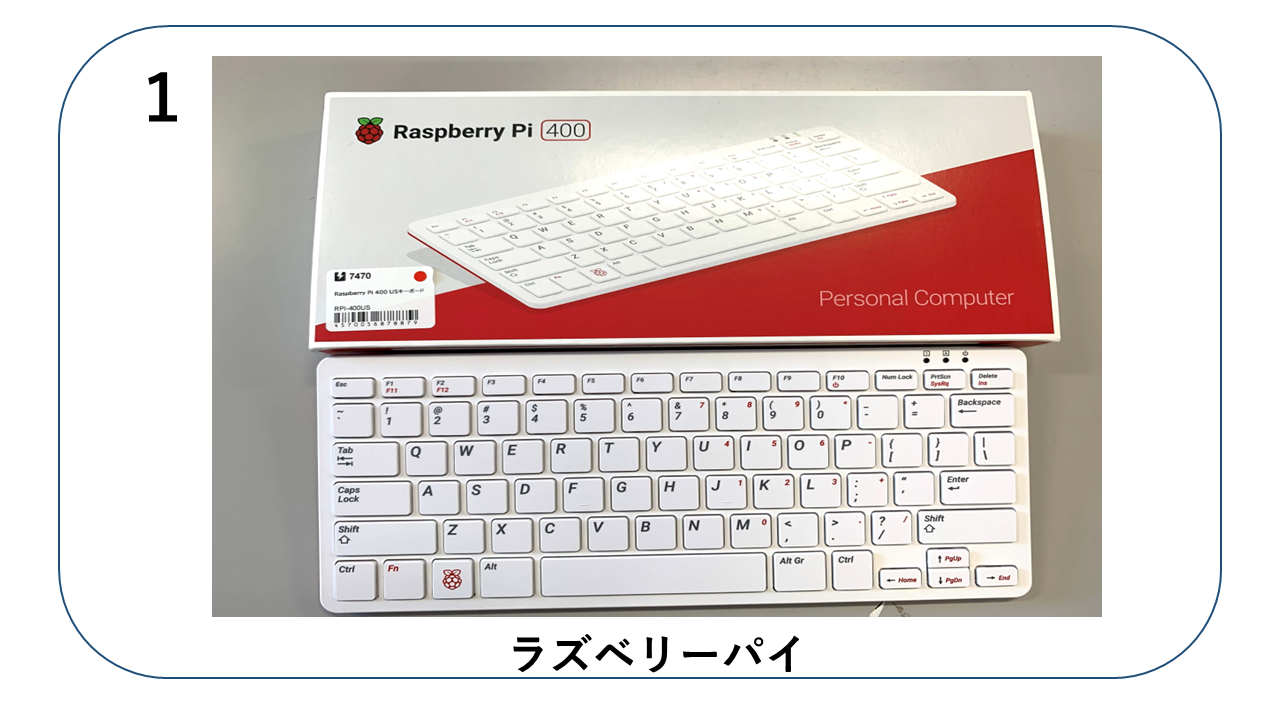
\includegraphics[width=6.488cm,height=4.697cm]{text01-img/textbook-img009-2023.png}
   &
  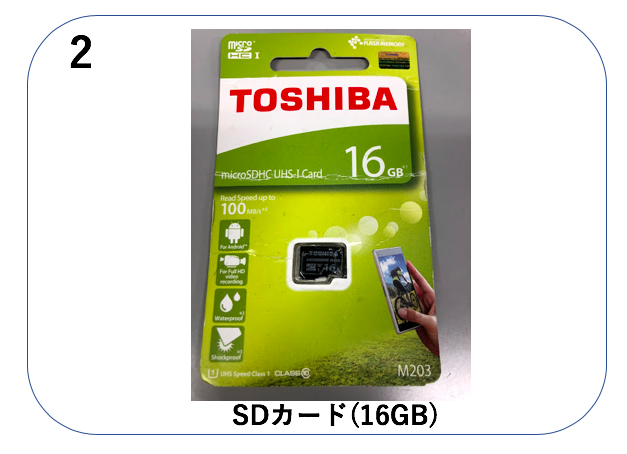
\includegraphics[width=6.488cm,height=4.697cm]{text01-img/textbook-img010.png} \\

  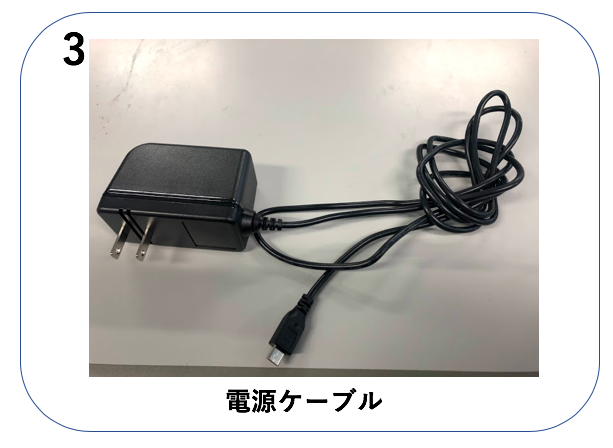
\includegraphics[width=6.488cm,height=4.697cm]{text01-img/textbook-img007.png}
   &
  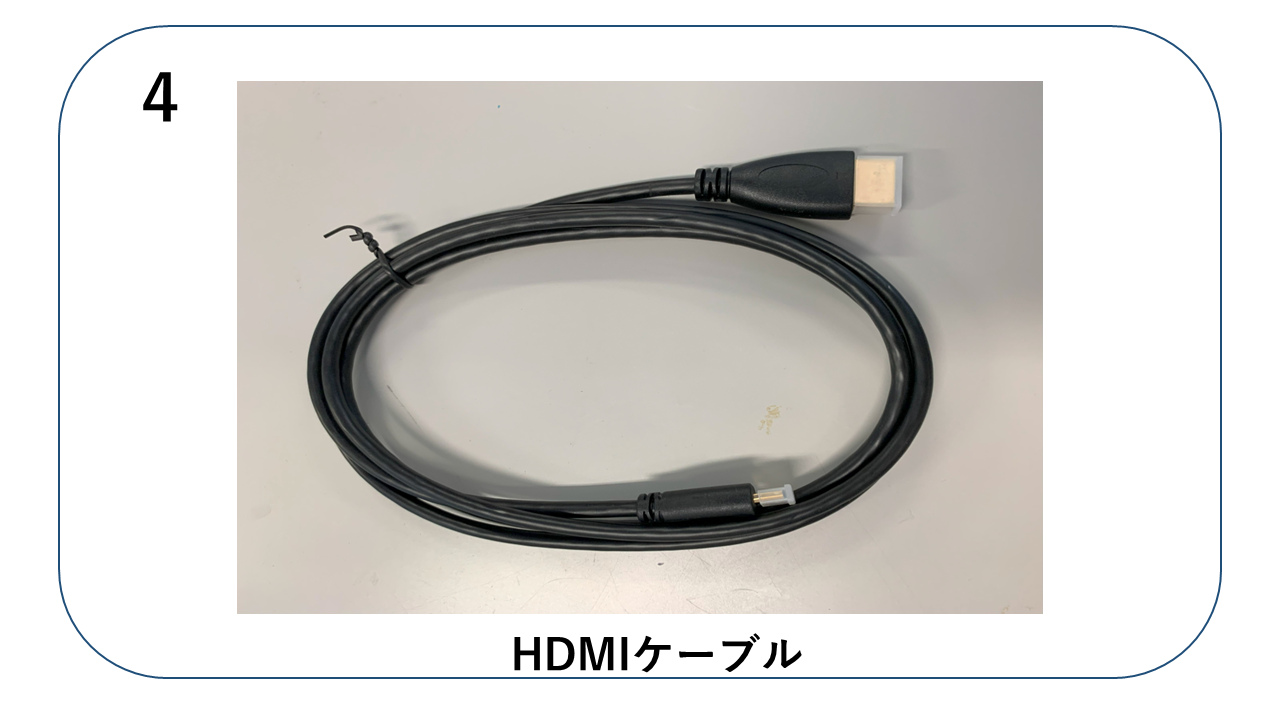
\includegraphics[width=6.488cm,height=4.697cm]{text01-img/textbook-img008-2023.png} \\

  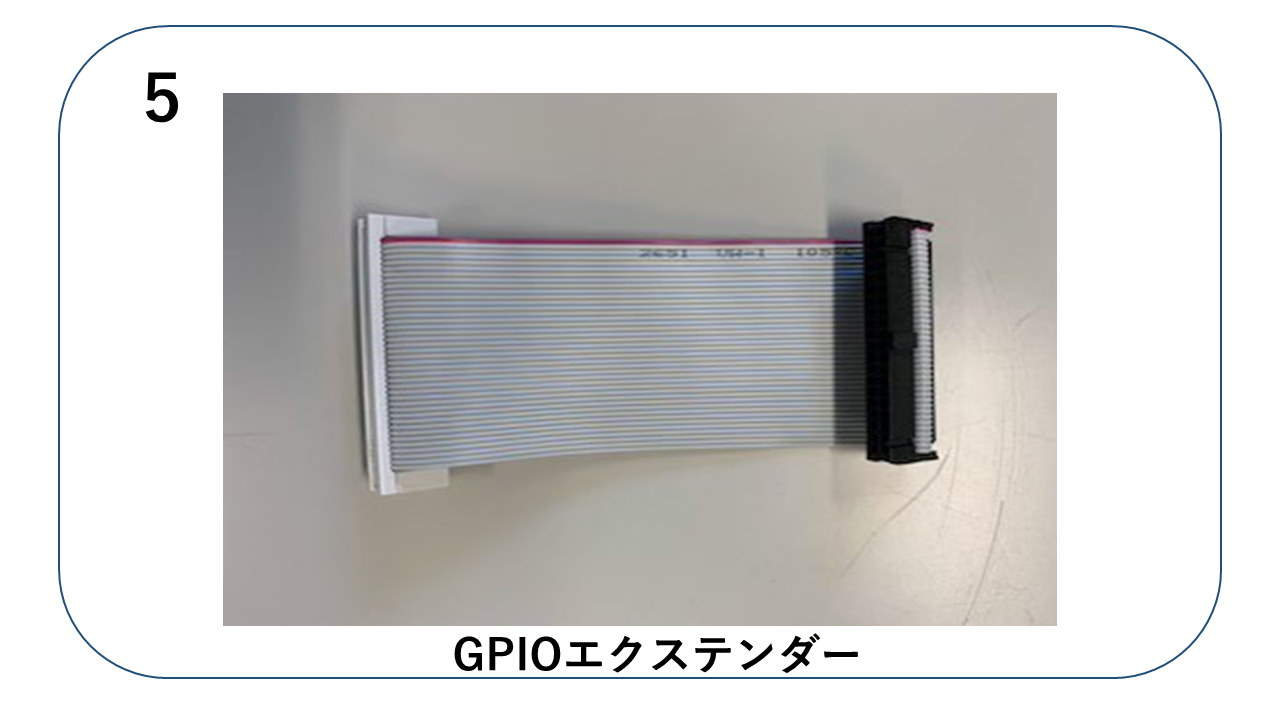
\includegraphics[width=6.488cm,height=4.697cm]{text01-img/textbook-img005-2023.png}
   &
  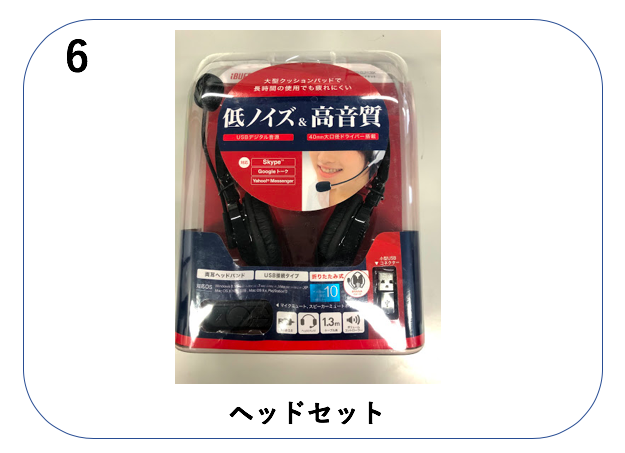
\includegraphics[width=6.488cm,height=4.697cm]{text01-img/textbook-img006.png}
\end{tabular}

\begin{tabular}{cc}

  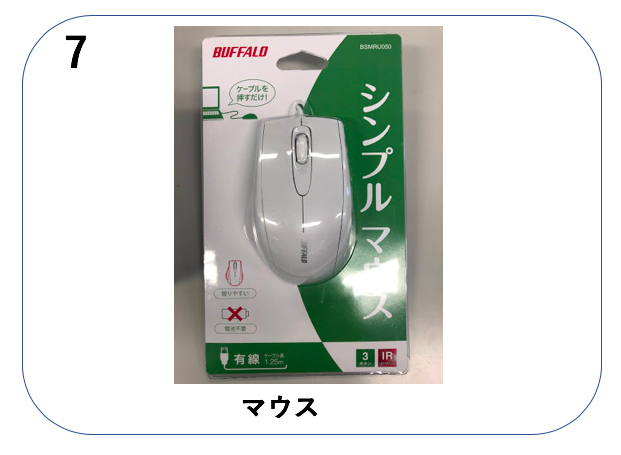
\includegraphics[width=6.488cm,height=4.697cm]{text01-img/textbook-img003.png}
   &
  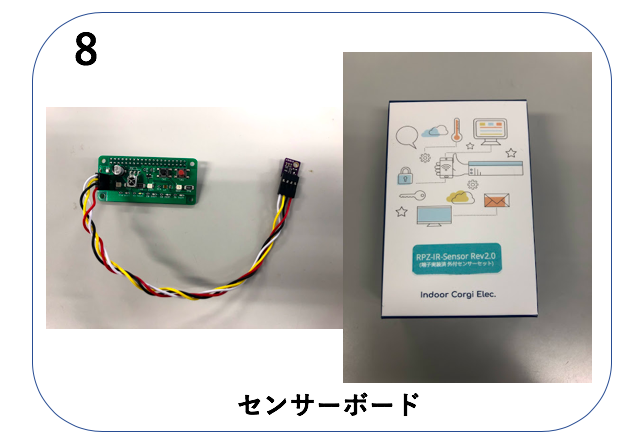
\includegraphics[width=6.488cm,height=4.697cm]{text01-img/textbook-img004.png}\\

  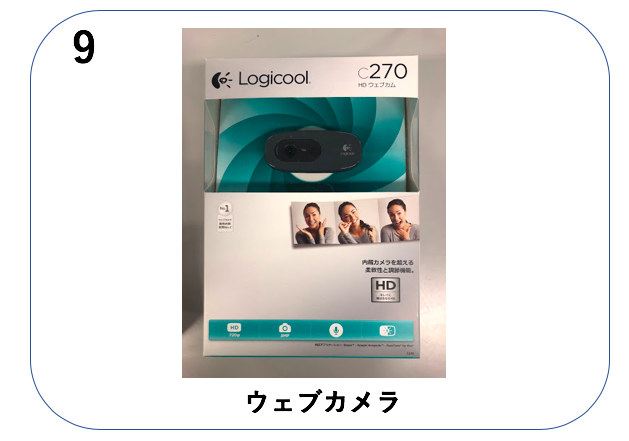
\includegraphics[width=6.488cm,height=4.697cm]{text01-img/textbook-img002.png}
   &
  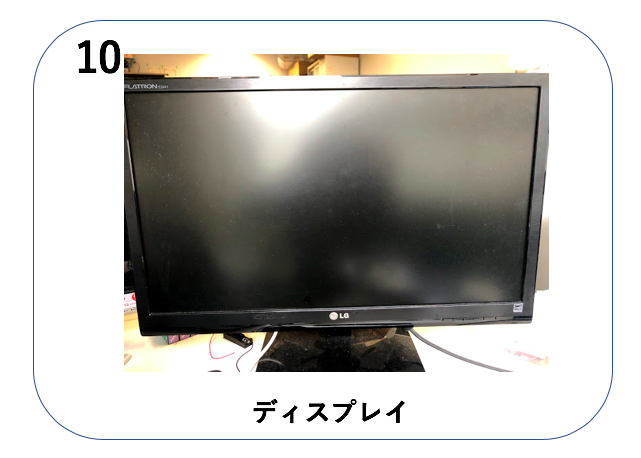
\includegraphics[width=6.488cm,height=4.697cm]{text01-img/textbook-img001.png} \\
\end{tabular}

% 
% subsection 1.1.6
% 
\subsection{ラズベリーパイについて}

イギリスのラズベリーパイ\ruby{財団}{ざいだん}が開発したコンピュータです。
いろいろな\ruby{種類}{しゅるい}がありますが、子どもIT\ruby{未来塾}{みらいじゅく}では
キーボード一体型のタイプを使用しています。
ラズベリーパイはラズパイとも\ruby{呼}{よ}ばれています。

% 
% subsection 1.1.7
% 
\subsection{\ruby{特徴}{とくちょう}}

\begin{itemize}
  \item キーボード一体型で、キーボードが必要ない
  \item \ruby{普通}{ふつう}のパソコンのように使える(動画\ruby{再生}{さいせい}やゲームもできます)
  \item プログラミングの\ruby{勉強}{べんきょう}に向いている
  \item モータやライトをせいぎょできる(目に見えるのでプログラミングを楽しめる)
\end{itemize}

% 
% subsection 1.1.8
% 
\subsection{ラズベリーパイでできること}

プログラミングを手軽に学ぶことができます。
プログラミングするにはパソコンが必要でお金もかかるため、やりたくてもできない人も
いたかもしれません。
しかし、ラズベリーパイのような小さくて手に入れやすいコンピュータがあれば手軽に
プログラミングの学習に取り組むことができます。
また、ラズベリーパイを使うことでモータを動かしたりライトを光らせたりすることができます。
これらのせいぎょをプログラムで行うことができるため、楽しみながら学習を進められます。

% 
% subsection 1.1.9
% 
\subsection{ラズベリーパイを使うときの注意}

\begin{itemize}
  \item 水などぬれているものをラズベリーパイ本体につけないようにしましょう
  \item ラズベリーパイ(コンピュータなど)は熱に弱いのですごく暑い部屋では使わないようにしましょう
  \item ラズベリーパイなどは静電気によわいので注意しましょう
  \item ラズベリーパイをらんぼうに\ruby{扱}{あつか}うのはやめましょう
\end{itemize}
\clearpage

% 
% subsection 1.1.10
% 
\subsection{パスワードについて学ぼう}

\begin{enumerate}
  % 1
  \item パスワードの\ruby{重要性}{じゅうようせい}について知ろう
  %
  \begin{itemize}
    \item IDとパスワードは、タブレットやパソコンなどの\ruby{情報機器}{じょうほうきき}や、
    インターネット上のサービスを利用する\ruby{際}{さい}に、\ruby{許可}{きょか}された者であるかを\ruby{識別}{しきべつ}し、
    本人を\ruby{確認}{かくにん}するための重要な\ruby{情報}{じょうほう}です。
    いわゆるインターネットやパソコンなどの電子機器に入るための\ruby{鍵}{かぎ}の名前(ユーザーID)と
    その\ruby{鍵}{かぎ}(パスワード)のようなものです。
    \begin{figure}[h]
      \centering
      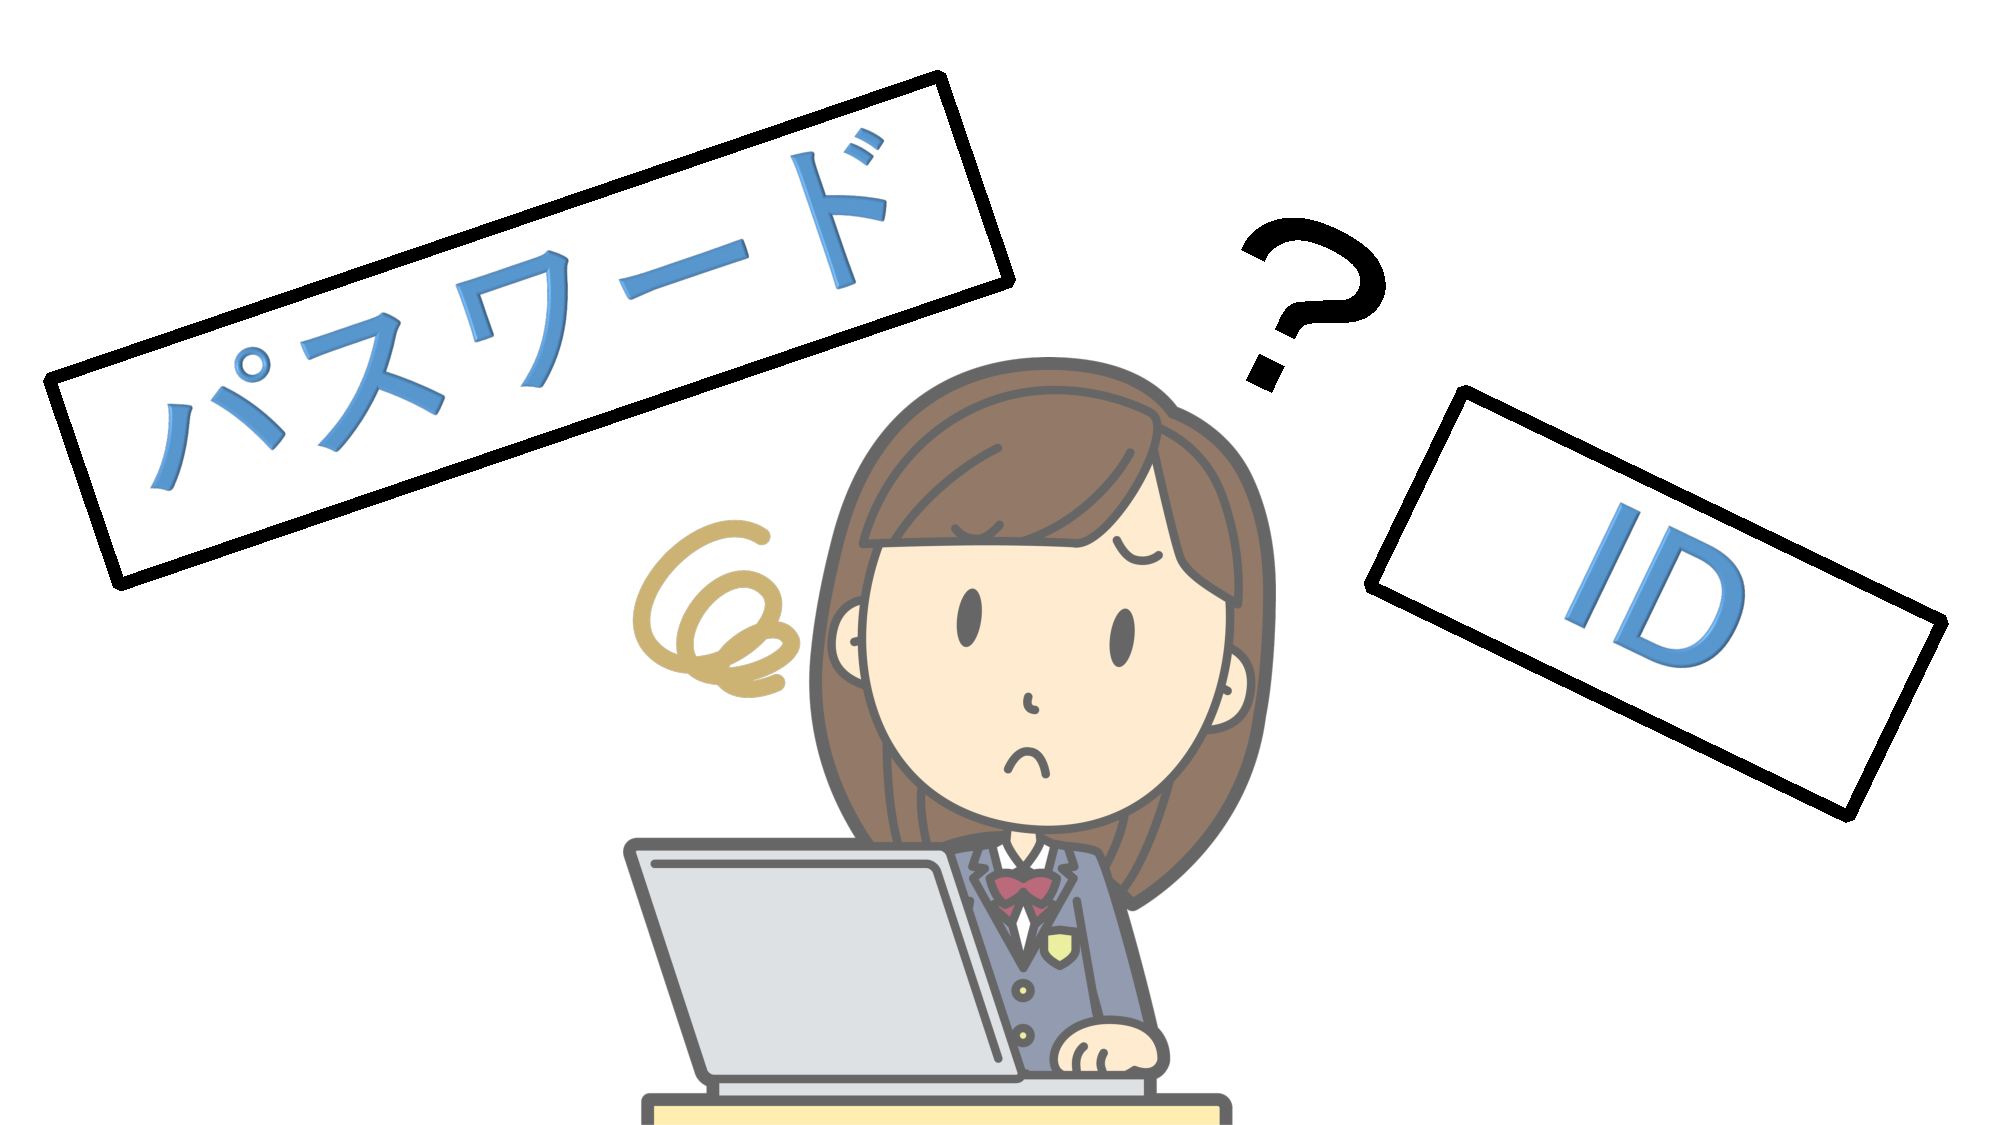
\includegraphics[width=7.000cm]{text01-img/pswd_image_imp6.pdf}
    \end{figure}

    \item IDやパスワードなど\ruby{認証}{にんしょう}で使っている\ruby{情報}{じょうほう}
    (\ruby{身分証明書}{みぶんしょうめいしょ})を\ruby{不適切}{ふてきせつ}な管理や、
    \ruby{攻撃}{こうげき}などで\ruby{盗}{ぬす}まれてしまうと、なりすましなどの\ruby{不正行為}{ふせいこうい}が
    行われてしまう\ruby{危険性}{きけんせい}もあります。
    \begin{figure}[h]
      \centering
      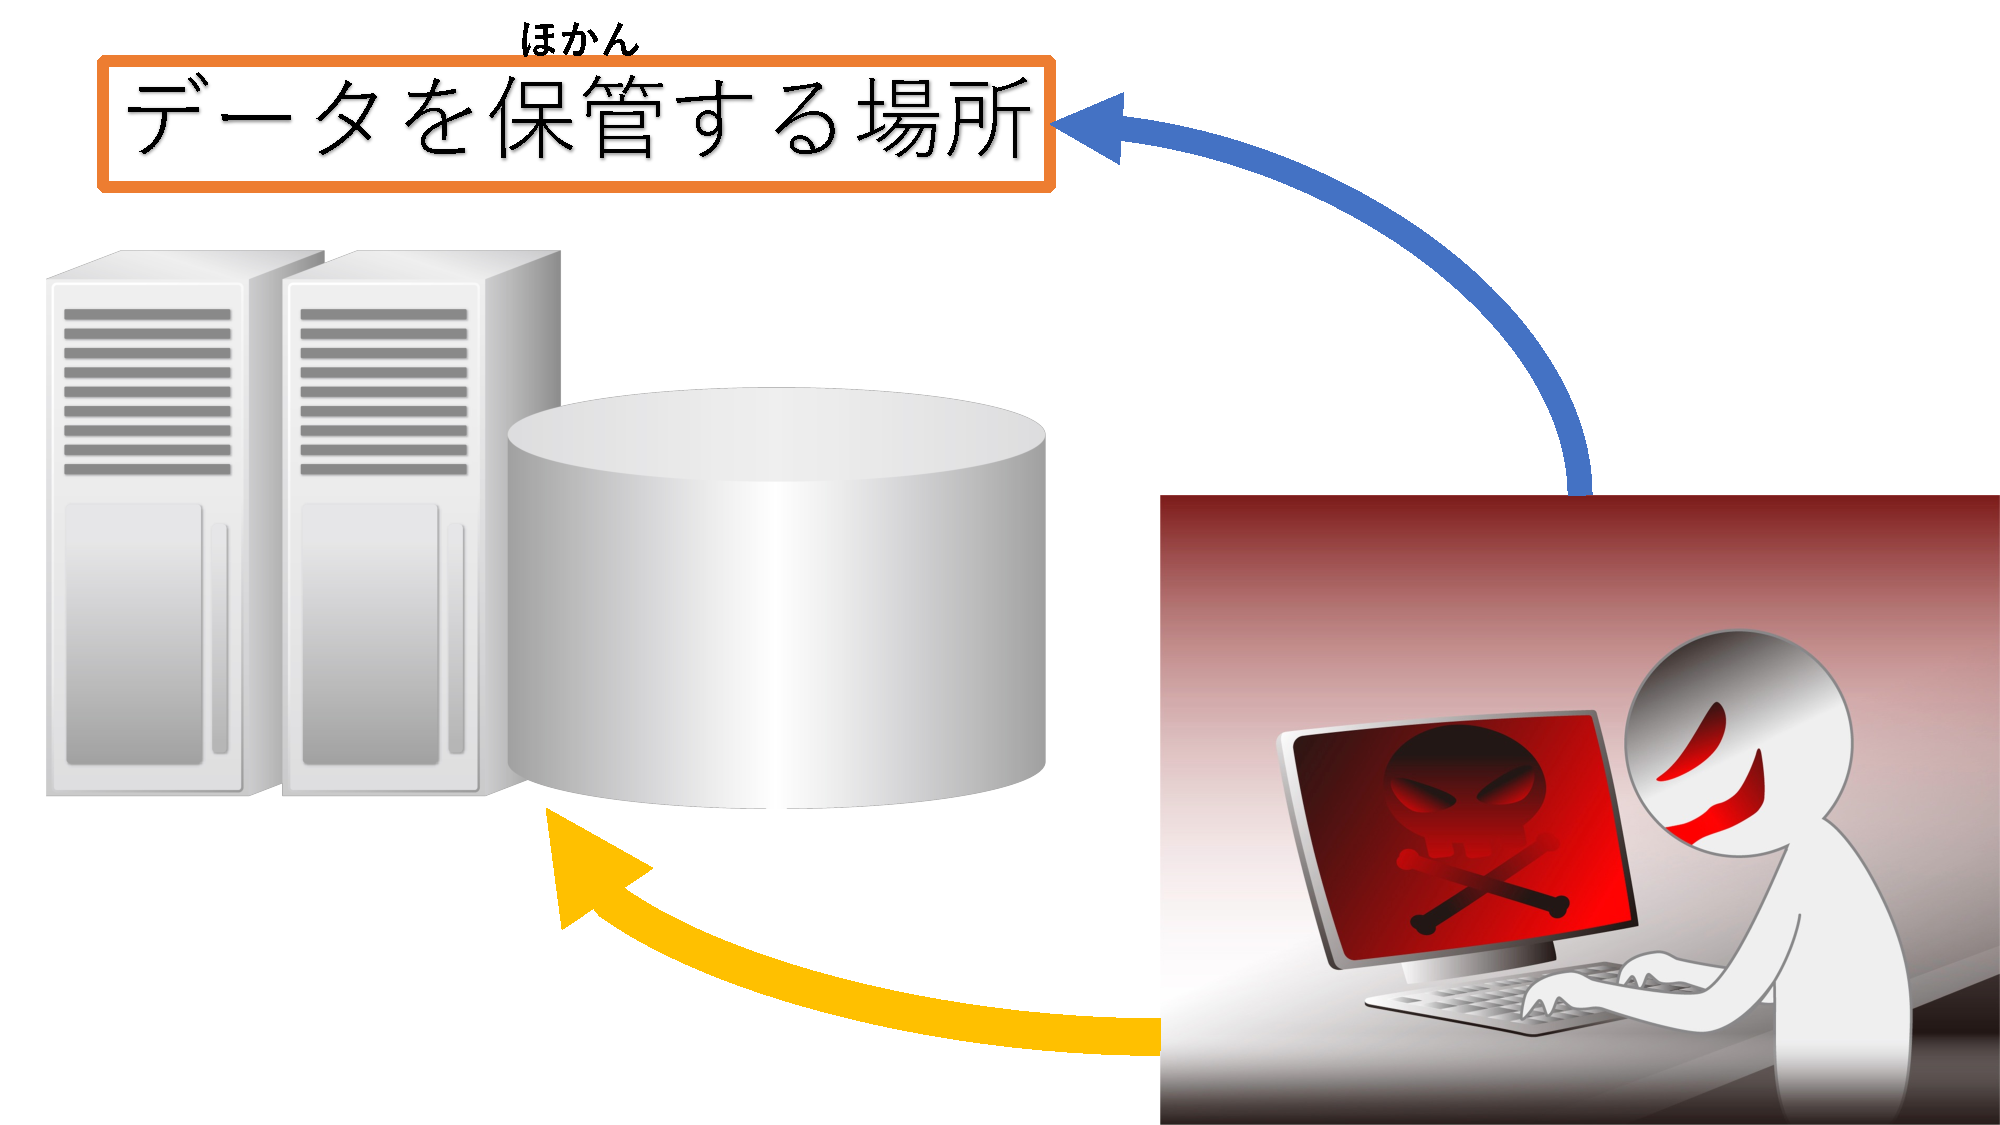
\includegraphics[width=7.000cm]{text01-img/pswd_image_imp5.pdf}
    \end{figure}

    \item このような手口による\ruby{被害}{ひがい}にあわないように、\ruby{認証}{にんしょう}の仕組みと
    \ruby{重要性}{じゅうようせい}を\ruby{理解}{りかい}して、IDやパスワードを\ruby{厳重}{げんじゅう}に管理しましょう。
    \begin{figure}[h]
      \centering
      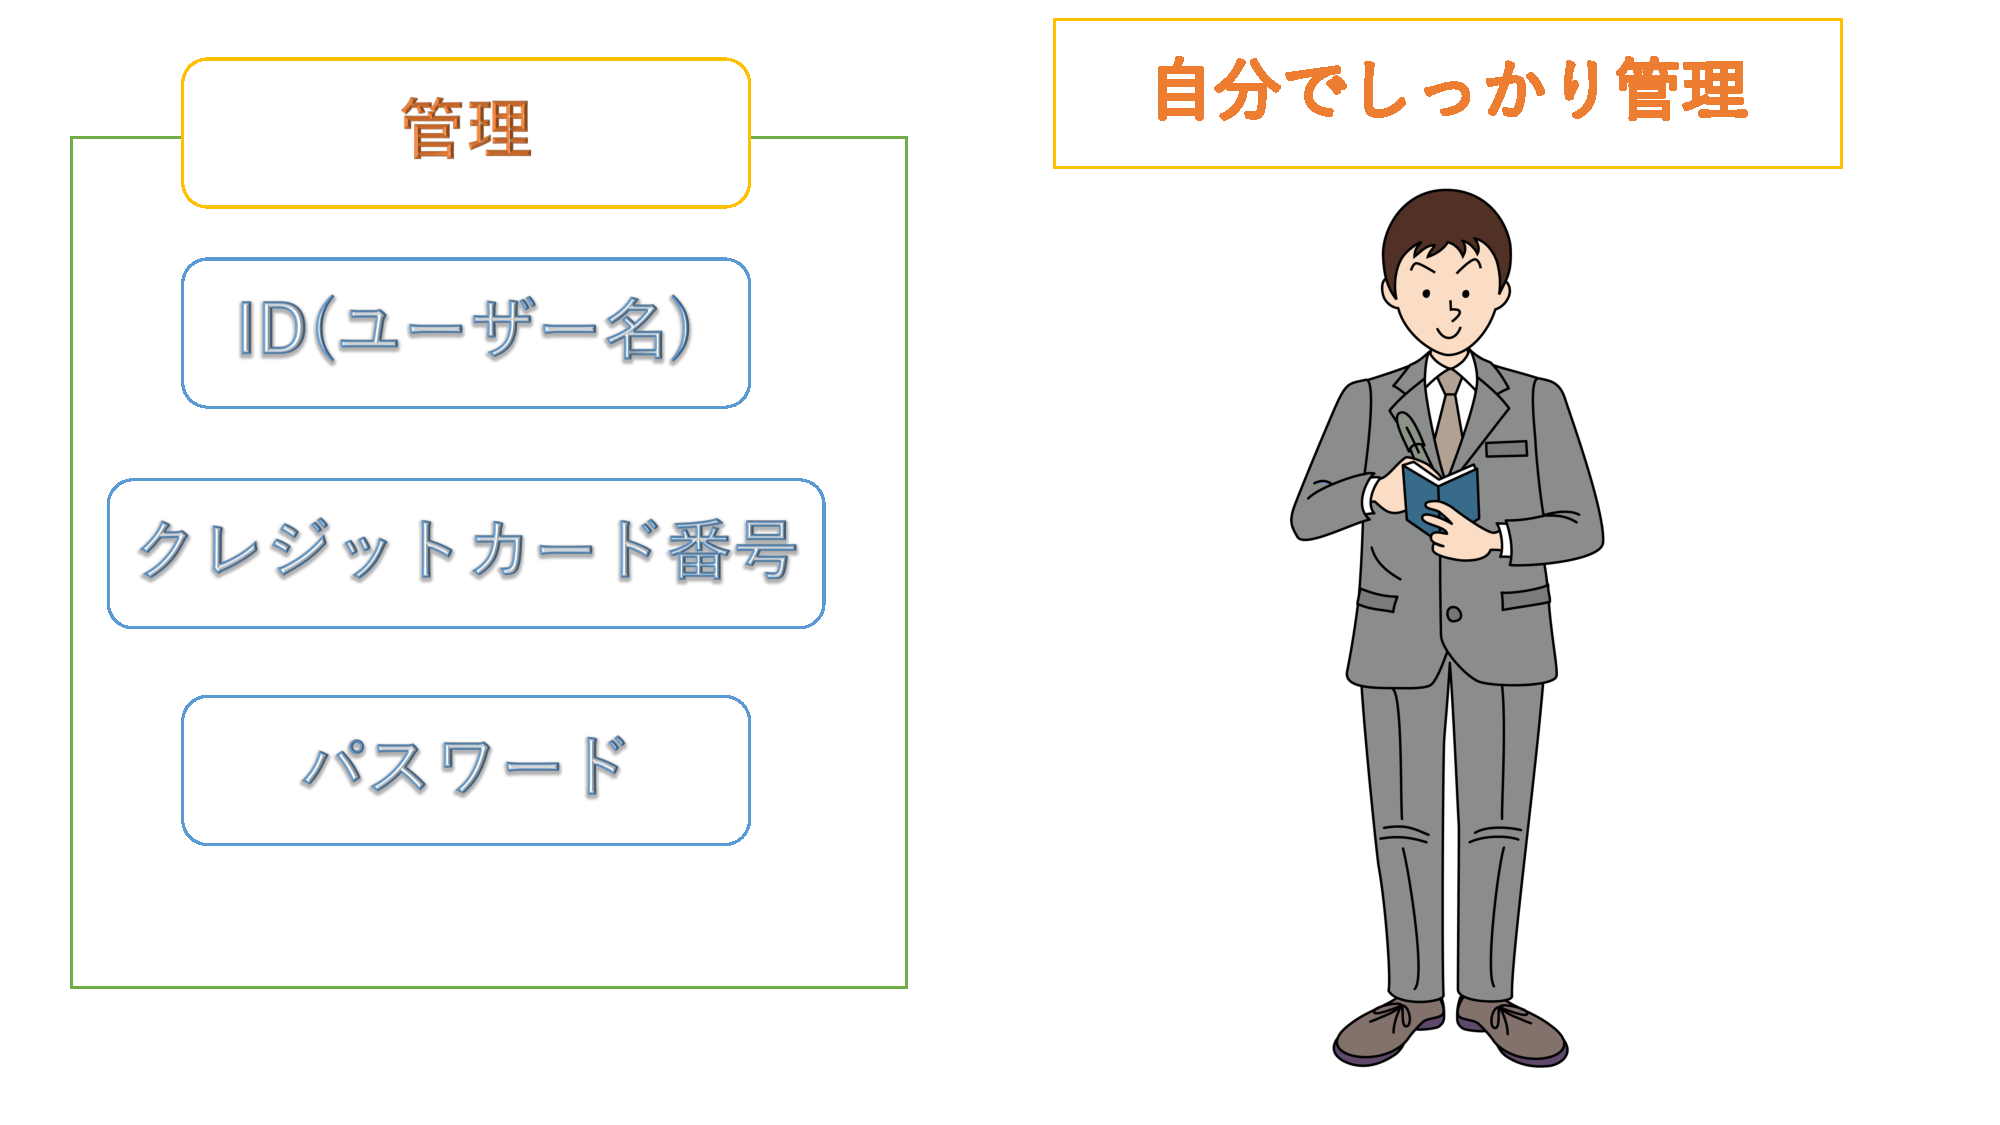
\includegraphics[width=7.000cm]{text01-img/pswd_image_imp3.pdf}
    \end{figure}
  \end{itemize}

\clearpage

  % 2
  \item 安全なパスワードの\ruby{設定}{せってい}やパスワードの\ruby{適切}{てきせつ}な管理について知ろう。
  
  \begin{itemize}
    \item 安全なパスワードとは他人に\ruby{推測}{すいそく}されにくく、計算で\ruby{割}{わ}り出しにくいものです。
  
    \begin{itemize}
      \item 名前などの\ruby{個人情報}{こじんじょうほう}からは\ruby{推測}{すいそく}できないこと
      \item 英単語などをそのまま使用していないこと
      \item アルファベットと数字が\ruby{混在}{こんざい}していること
      \item \ruby{適切}{てきせつ}な長さの文字列であること
      \item \ruby{類推}{るいすい}しやすい\ruby{並}{なら}び方やその\ruby{安易}{あんい}な組合せにしないこと
    \end{itemize}

    \begin{figure}[h]
      \centering
      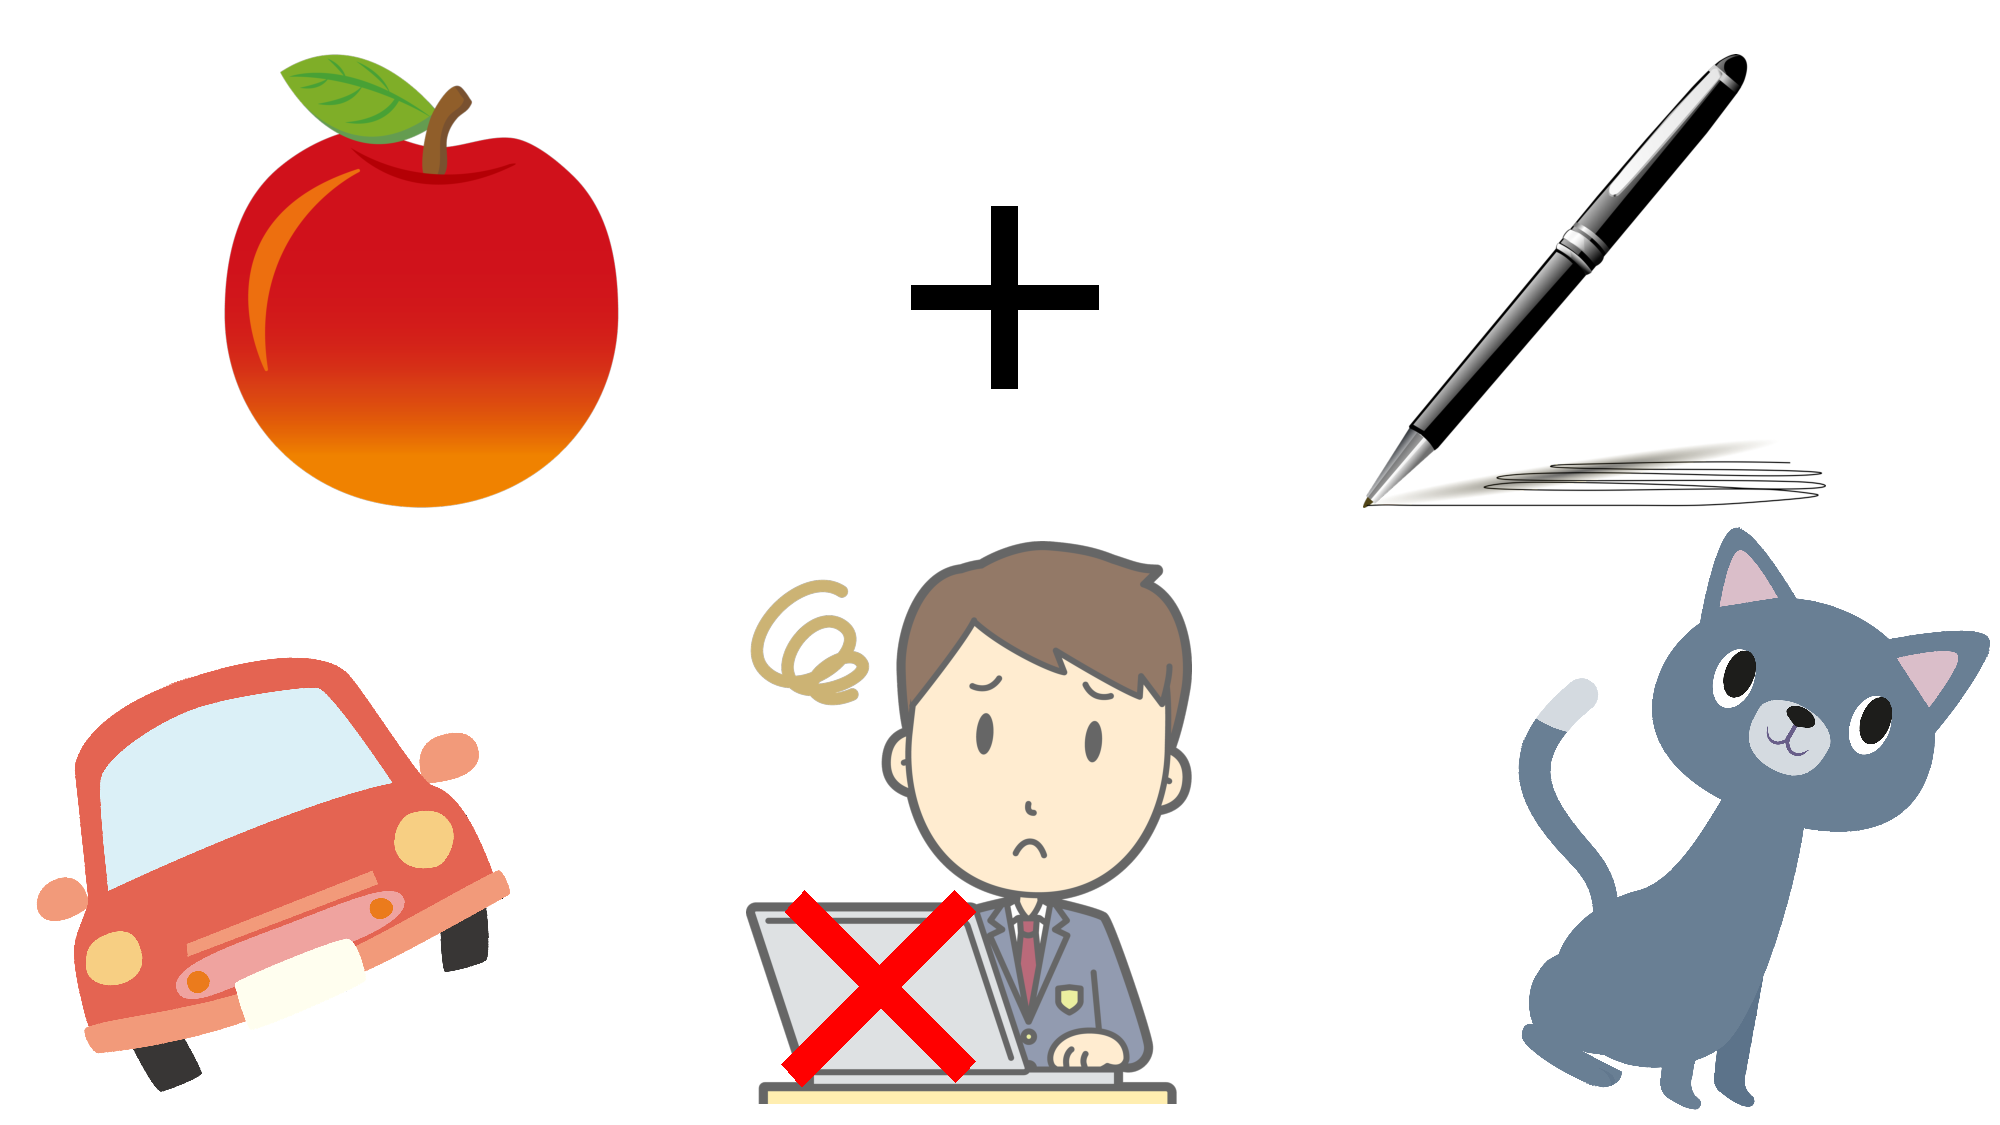
\includegraphics[width=7.000cm]{text01-img/pswd_image_imp11.pdf}
    \end{figure}

    \item パスワードはできる限り、\ruby{複数}{ふくすう}のサービスで使い回さないようにしましょう。またパスワードを定期的に\ruby{変更}{へんこう}することを求められても、\ruby{実際}{じっさい}にパスワードを\ruby{破}{やぶ}られアカウントが乗っ取られたり、サービス側から流出した事実がなければパスワードを\ruby{変更}{へんこう}する必要はありません。
    \begin{figure}[h]
      \centering
      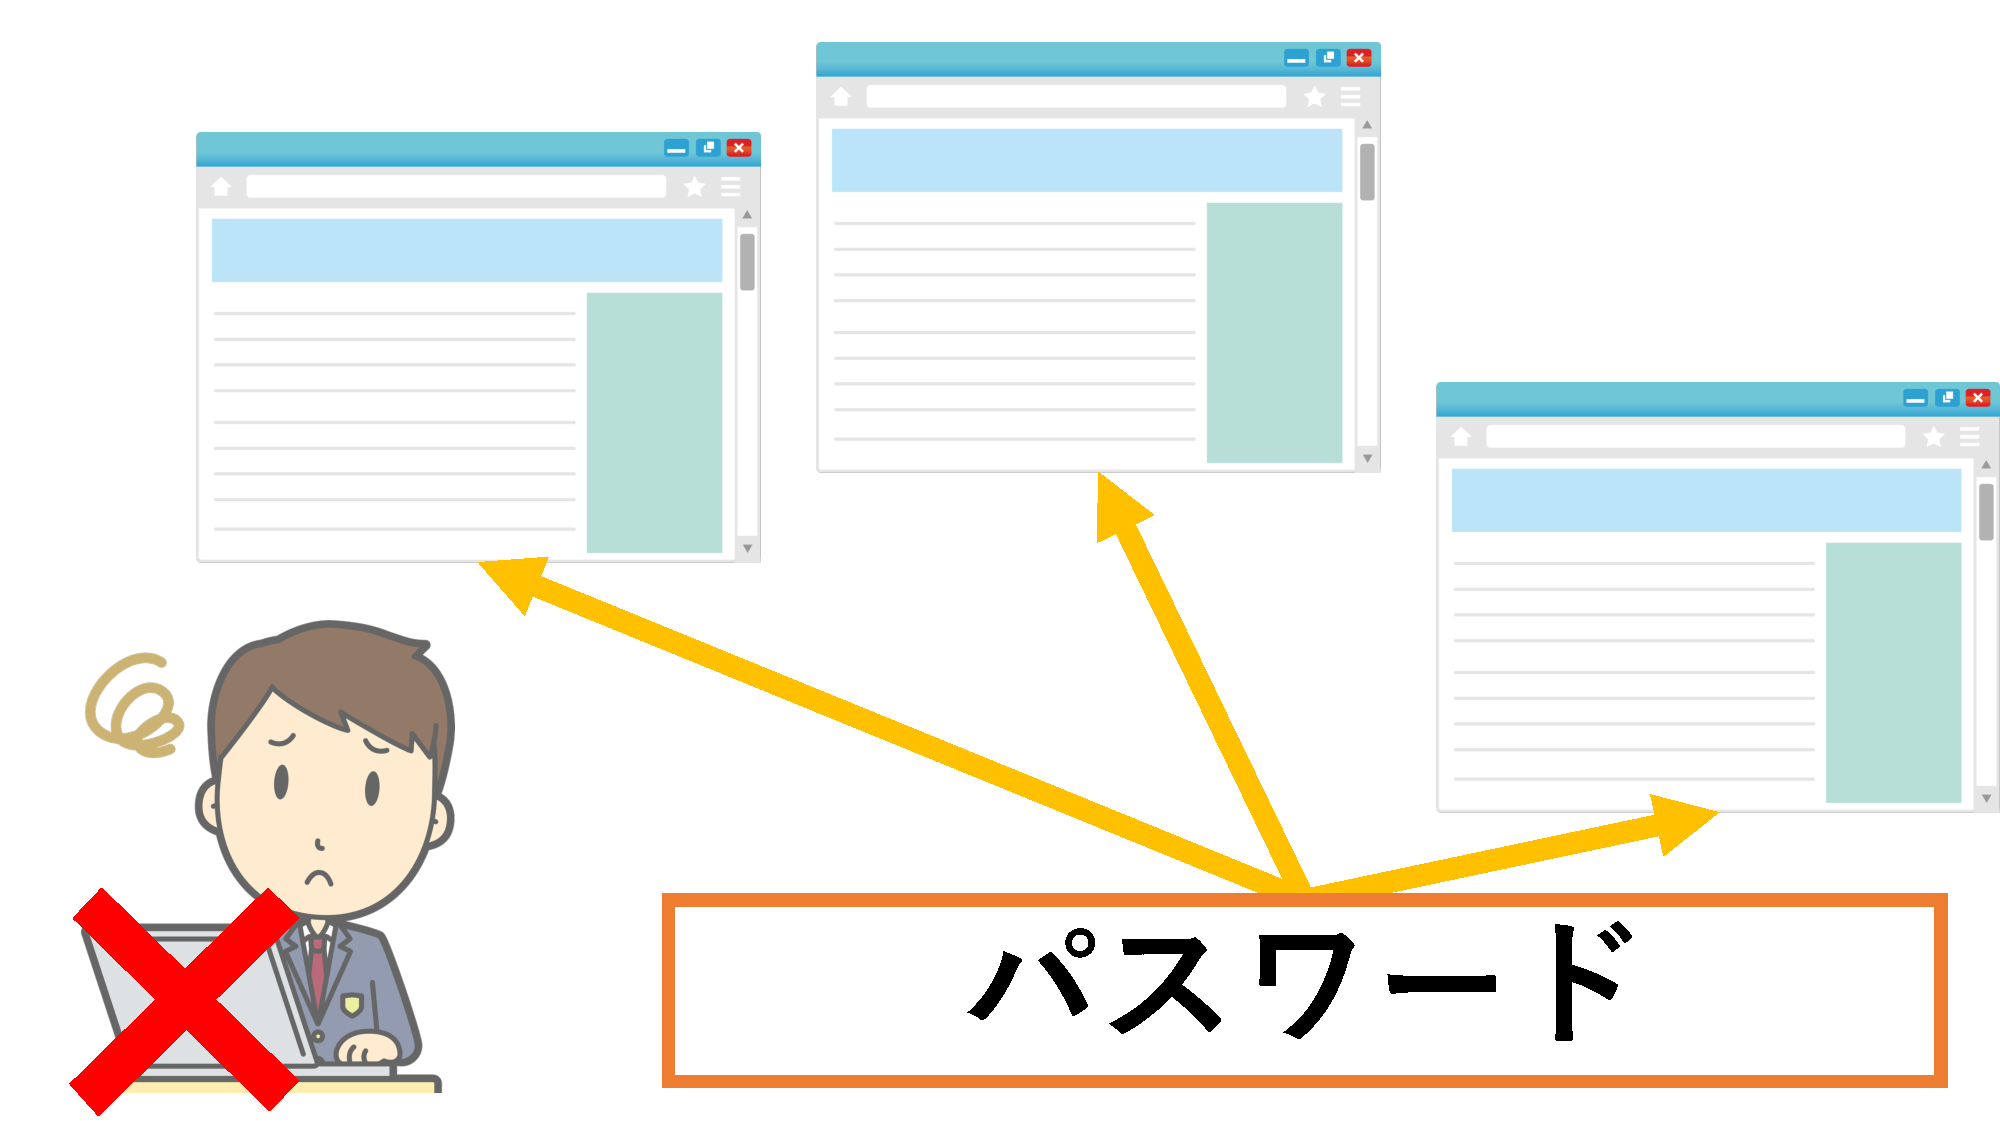
\includegraphics[width=7.000cm]{text01-img/pswd_image_imp10.pdf}
    \end{figure}

    \item 安全なパスワードを\ruby{設定}{せってい}してもパスワードが他人に\ruby{漏}{も}れてしまえば意味がありません。
    以下に関して特に\ruby{留意}{りゅうい}が必要です。

    \begin{itemize}
      \item パスワードは友人などに教えずに\ruby{秘密}{ひみつ}にすること
      \item パスワードをメールやSNSなどでやりとりしないこと
      \item パスワードのメモなどを他人の目に付く場所に\ruby{貼}{は}ったり置いたりしないこと
      \item パスワードをメモした場合は\ruby{鍵}{かぎ}のかかる\ruby{机}{つくえ}や金庫など安全に\ruby{保管}{ほかん}すること
    \end{itemize}
    \bigskip

    \item 出典: \ruby{総務省}{そうむしょう}『国民のための\ruby{情報}{じょうほう}セキュリティサイト』
    \url{https://www.soumu.go.jp/main_sosiki/joho_tsusin/security/basic/privacy/01-1.html}を加工して作成
  \end{itemize}
  \clearpage

  % 3
  \item パスワードの\ruby{制限}{せいげん}について知ろう
  
  \begin{itemize}
    \item Linuxのユーザー名とパスワードの\ruby{入力基準}{にゅうりょくきじゅん}において以下の\ruby{条件}{じょうけん}があります。

    \begin{itemize}
      \item ユーザー名は小文字、数字、-、のみ使用\ruby{可能}{かのう}
      \item パスワードは8文字以上16文字以下
      \item パスワードには以下の四つのカテゴリタイプの文字の内、三つのカテゴリタイプの文字を入れる必要がある
    \end{itemize}

    \begin{table}[htbp]
      \centering
      \caption{文字タイプ表}
      \begin{tabular}{|c|c|}
      \hline
          タイプ & \ruby{実際}{じっさい}に使用\ruby{可能}{かのう}な文字 \\
          \hline
          大文字& \verb|ABCDEFGHIJKLMNOPQRSTUVWXYZ| \\
          \hline
          小文字& \verb|abcdefghijklmnopqrstuvwxyz| \\
          \hline
          数字 & \verb|0123456789| \\
          \hline
          英数字以外の文字 & \verb|!@#$%^&*()_+`{}[]\:";'<>?,./| \textbar\\
          \hline
      \end{tabular}
    \end{table}

    \item \ruby{注意事項}{ちゅういじこう}
    
    \begin{itemize}
      \item パスワードの先頭の大文字とパスワードの\ruby{末尾}{まつび}の数字は、使用される文字クラスの数にはカウントされません
      \item パスワードには辞書の単語やユーザーのログイン名を\ruby{含}{ふく}めることはできません
      \item 文字を数字または英数字以外の文字に置き\ruby{換}{か}えると、辞書の単語が受け入れられるようになります
      (例)\verb+app1e+, \verb+ta2ya+
      \item なるべく自分が覚えやすいものにしてください。
      ※\ruby{公}{おおやけ}になっている\ruby{羅列}{られつ}やその他ですでに使用しているものは\ruby{避}{さ}けてください 
    \end{itemize}

  \end{itemize}
  \vskip\baselineskip

  \begin{itemize}
    \item \textbf{問題 1-1} パスワードとユーザ名を決めて下の\ruby{記入欄}{きにゅうらん}に記入してみましょう。
    \vskip\baselineskip
    \vskip\baselineskip
    \vskip\baselineskip
    \vskip\baselineskip
    \underline{ユーザ名(ID):\hspace{10.8cm}}
    \vskip\baselineskip
    \vskip\baselineskip
    \vskip\baselineskip
    \vskip\baselineskip
    \underline{パスワード:\hspace{11.3cm}}
    \vskip\baselineskip
  \end{itemize}
  \clearpage
  
  \begin{itemize}
    \item \textbf{問題 1-2} 次の文章で正しいものには〇を、\ruby{誤}{あやま}っているものには✕を記入してください。
  \end{itemize}
  \begin{description}
    \item (1) 名前などの\ruby{個人情報}{こじんじょうほう}からは\ruby{推測}{すいそく}でしやすい方が良い
    \item (2) 英単語などをそのまま使用して良い
    \item (3) \ruby{適切}{てきせつ}な長さの文字列である方が良い
    \item (4) \ruby{類推}{るいすい}しやすい\ruby{並}{なら}び方やその\ruby{安易}{あんい}な組合せが良い
  \end{description}

  \begin{table}[H]
    \centering
    \begin{tabular}{|c|}
      \hline
      {\LARGE (1)【\hspace{3pc}】(2)【\hspace{3pc}】(3)【\hspace{3pc}】(4)【\hspace{3pc}】}\\
      \hline
    \end{tabular}
  \end{table}
  % \clearpage

  % \begin{table}[htbp]
  %   \centering  
  %   \begin{tabular}{|c|c|c|}
  %   \hline
  %       番号&\ruby{訂正}{ていせい}する\ruby{箇所}{かしょ}&\ruby{訂正後}{ていせいご}  \\
  %       \hline
  %       例(1)& \ruby{推測}{すいそく}しやすい&\ruby{推測}{すいそく}しにくい\\
  %       \hline
  %       (2)& & \\
  %       \hline
  %       (3)& & \\
  %       \hline
  %       (4)& & \\
  %       \hline
  %   \end{tabular}
  % \end{table}

  \begin{itemize}
    \item \textbf{問題 1-3} 次の文章で正しいものには○を、\ruby{誤}{あやま}ってるものには×を記入してください。
  \end{itemize}

  \begin{description}
    \item (1) パスワードは友人などに教えずに\ruby{秘密}{ひみつ}にすること
    \item (2) パスワードを送る時はメールやSNSなどで送る
    \item (3) パスワードのメモなどを他人の目に付く場所に\ruby{貼}{は}ったり置いておく
    \item (4) パスワードをメモした場合は\ruby{鍵}{かぎ}のかかる\ruby{机}{つくえ}や金庫など安全に\ruby{保管}{ほかん}すること
  \end{description}

  \begin{table}[H]
    \centering
    \begin{tabular}{|c|}
      \hline
      {\LARGE (1)【\hspace{3pc}】(2)【\hspace{3pc}】(3)【\hspace{3pc}】(4)【\hspace{3pc}】}\\
      \hline
    \end{tabular}
  \end{table}

  \begin{itemize}
    \item \textbf{問題 1-4} 次のパスワードは\ruby{安全性}{あんぜんせい}が高いパスワードには○低いパスワードには×を記入しなさい。
  \end{itemize}

  \begin{description}
    \item  (1) Wp9jaFk6agkoa0la
    \item  (2) Abcdefg123456789
    \item  (3) AppleMan0101
    \item  (4) Kaei1
  \end{description}

  \begin{table}[H]
    \centering
    \begin{tabular}{|c|}
      \hline
      {\LARGE (1)【\hspace{3pc}】(2)【\hspace{3pc}】(3)【\hspace{3pc}】(4)【\hspace{3pc}】}\\
      \hline
    \end{tabular}
  \end{table}

\end{enumerate}

\clearpage

% \begin{enumerate}

% 
% subsection 1.1.11
% 
\subsection{ラズベリーパイを\ruby{準備}{じゅんび}しよう(手順)}

ラズベリーパイとマウス等を\ruby{接続}{せつぞく}して起動する\ruby{準備}{じゅんび}をします。

\begin{figure}[H]
  \centering
  % 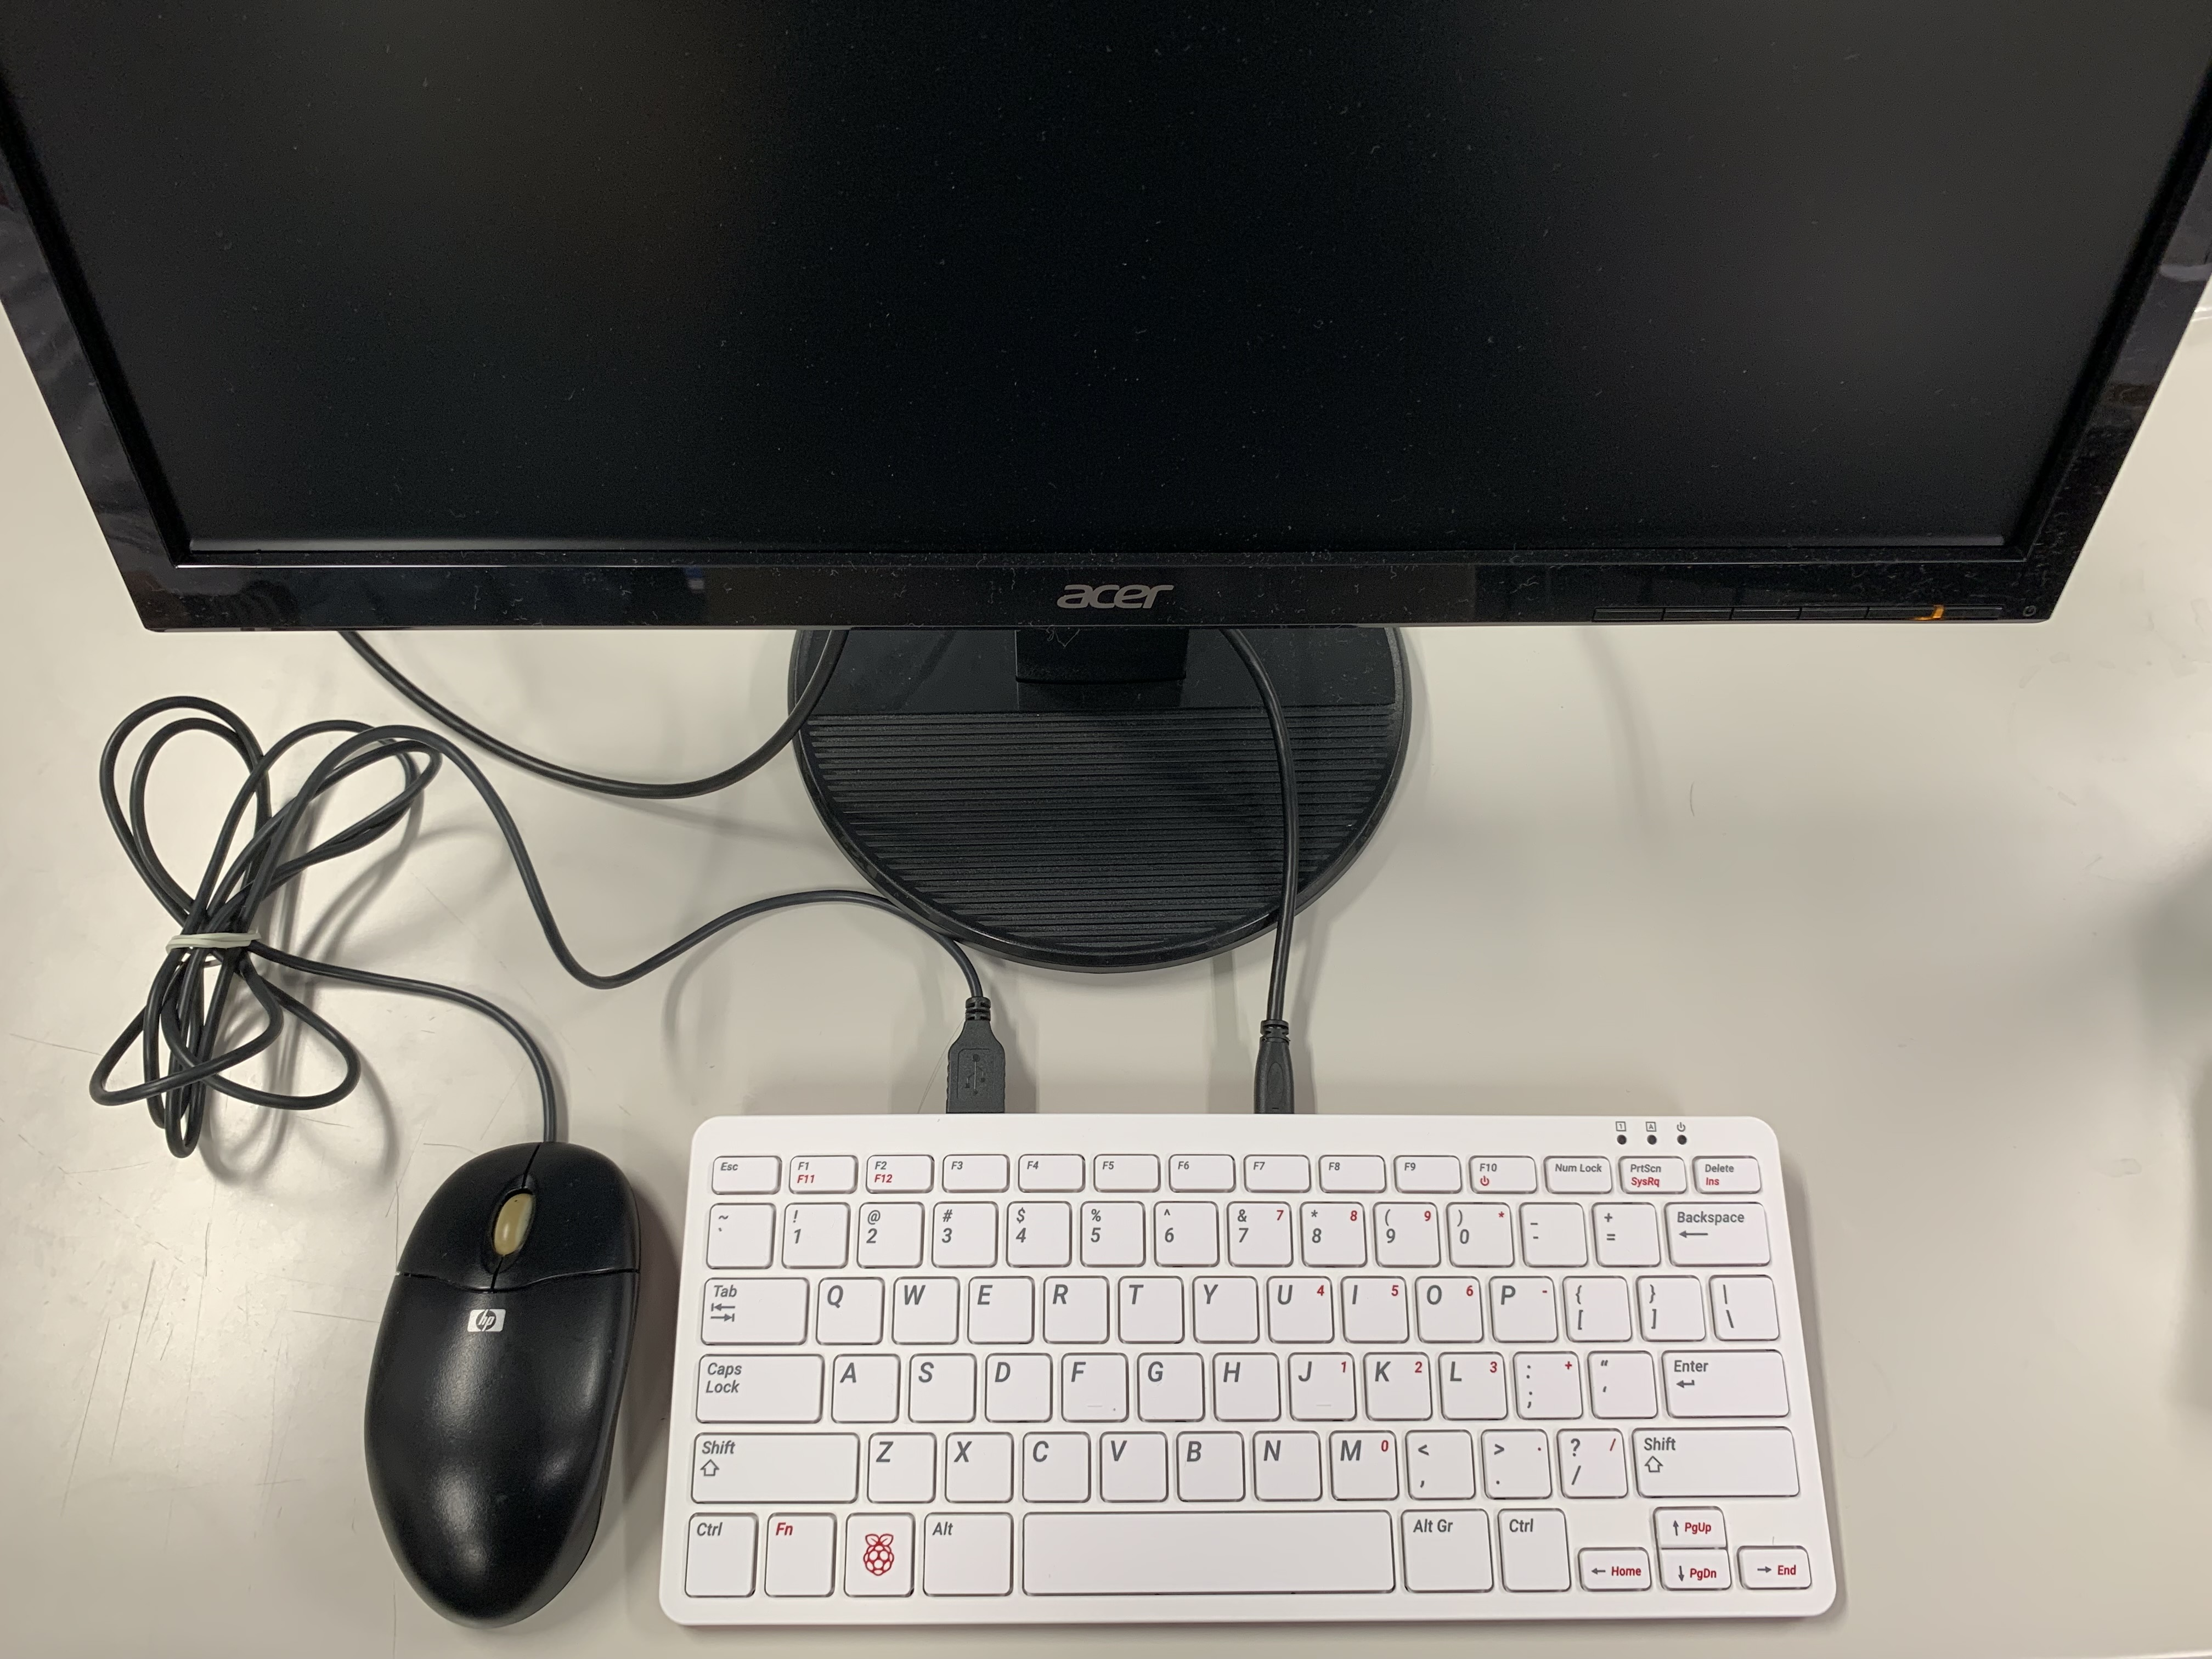
\includegraphics[keepaspectratio,width=11.232cm,height=8.424cm]{text01-img/connections01-2023.jpg}
  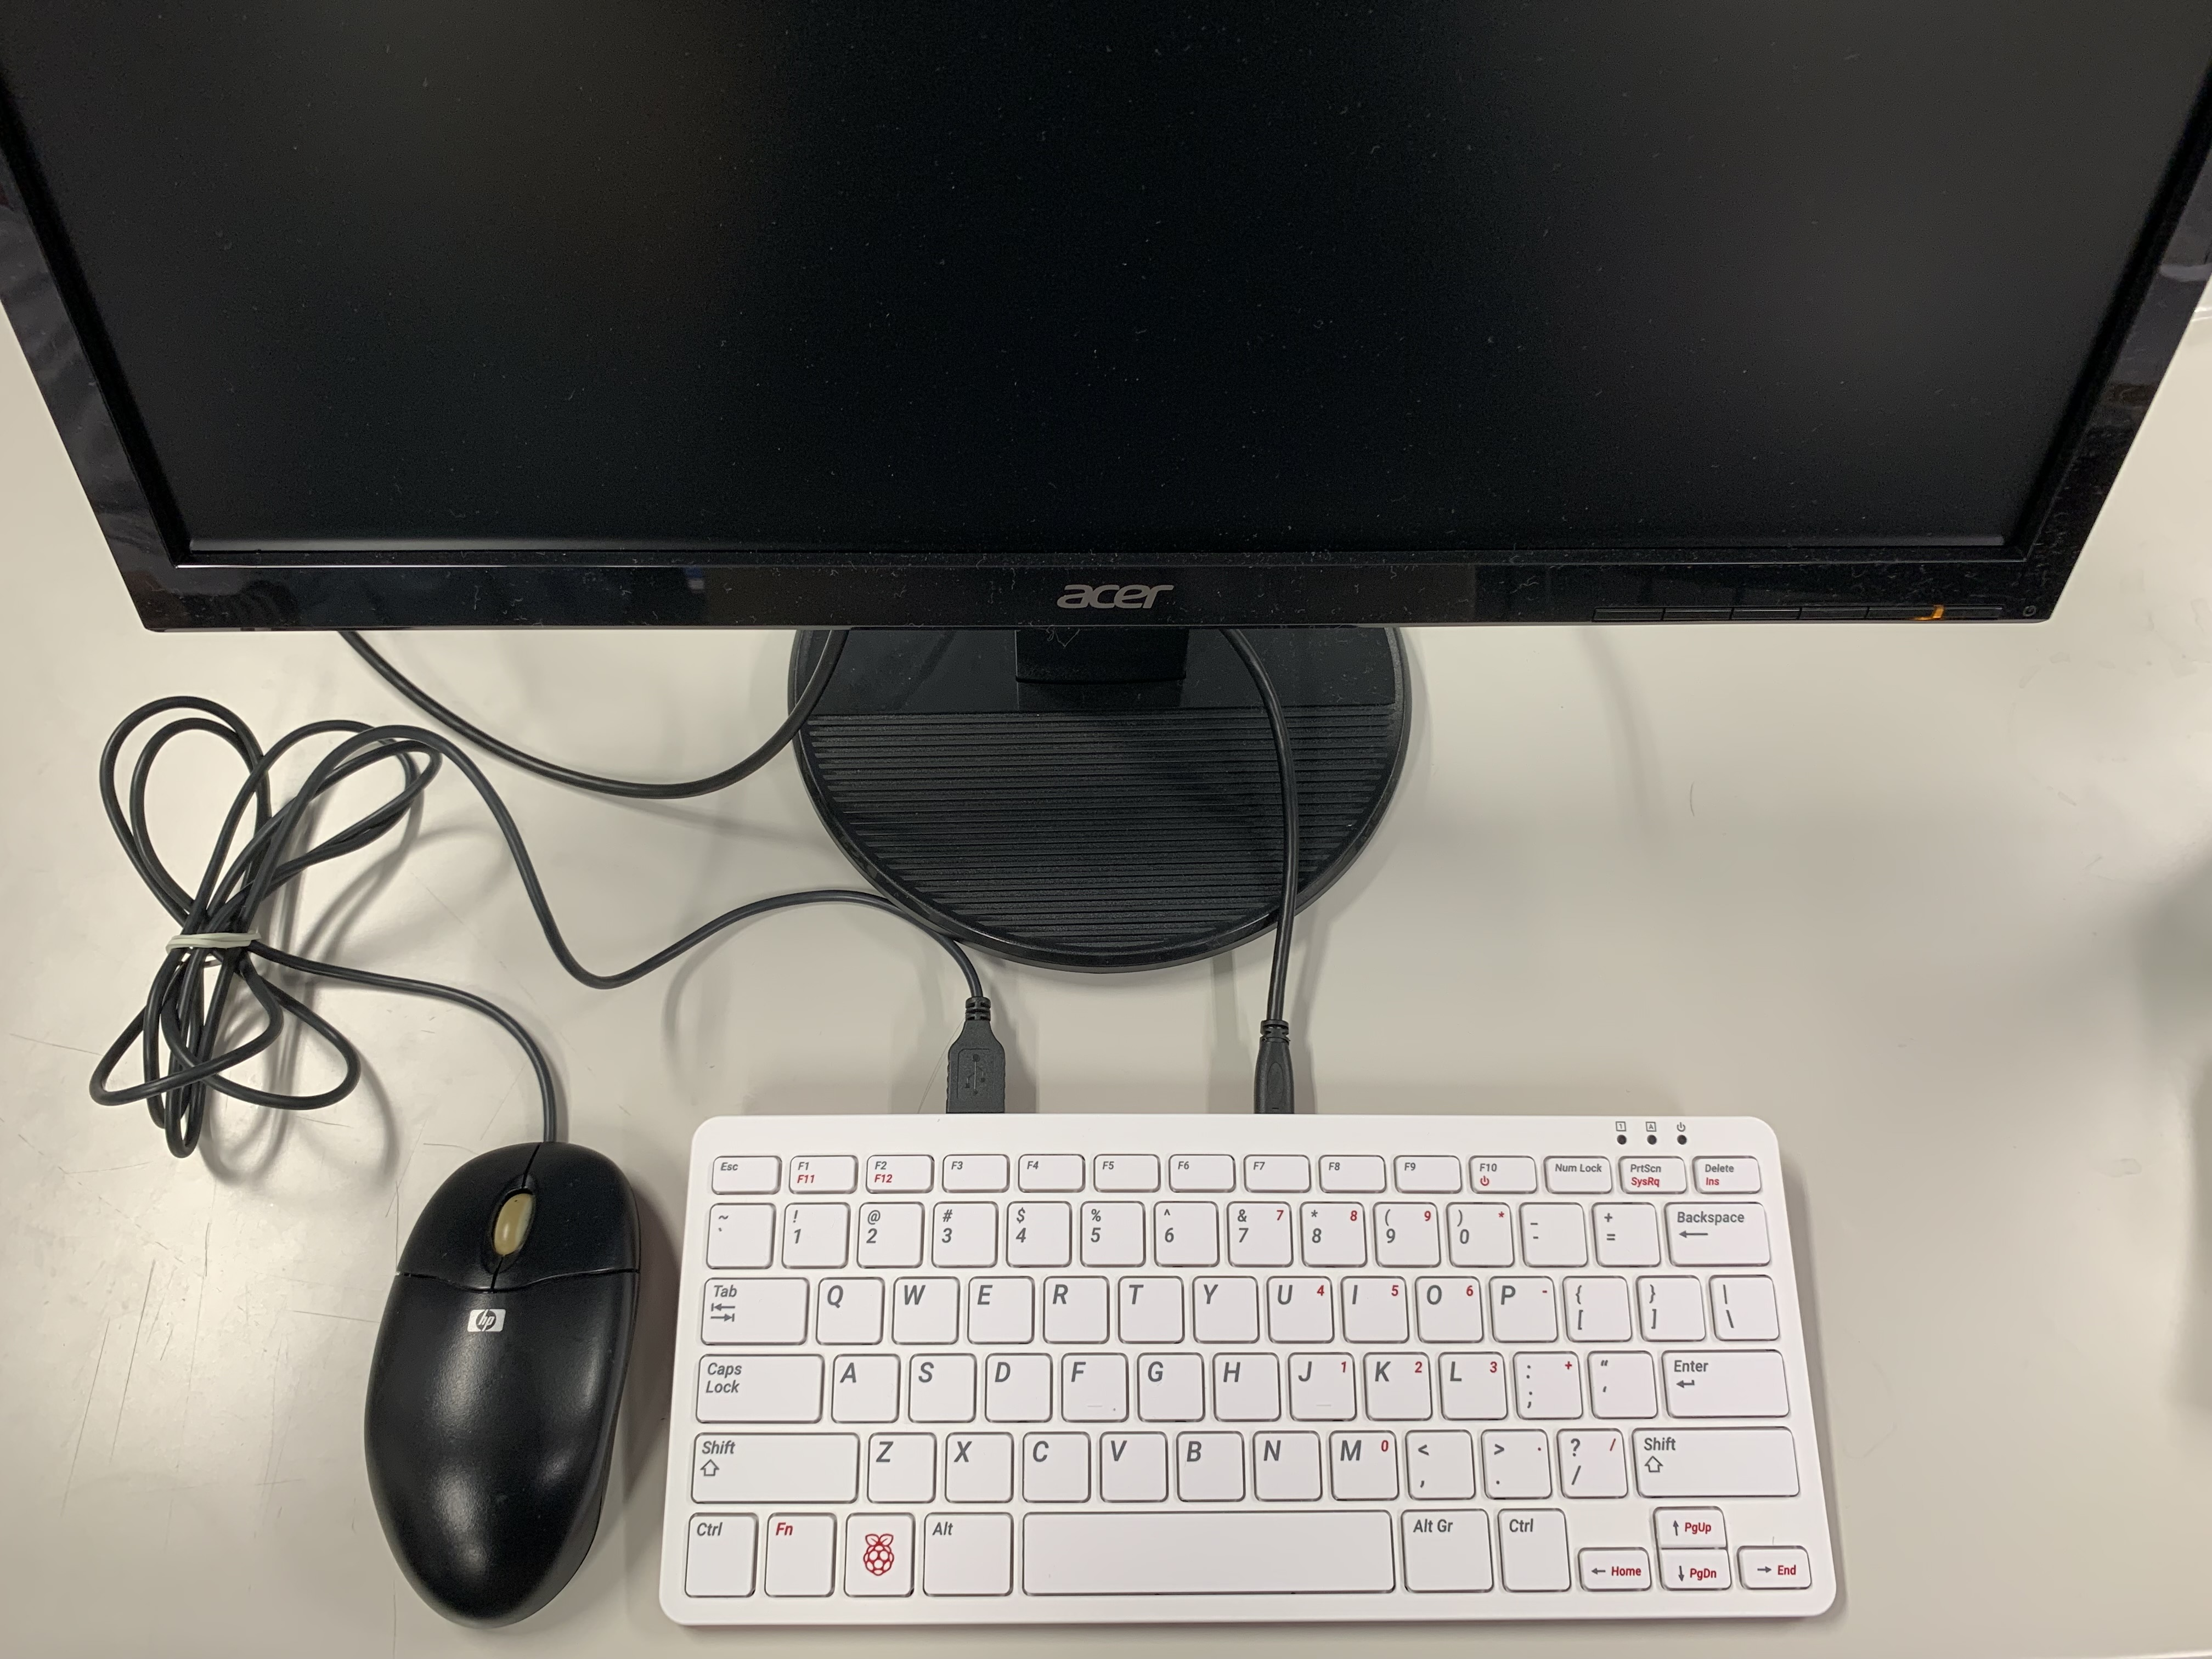
\includegraphics[keepaspectratio,height=7cm]{text01-img/connections01-2023.jpg}
  \caption{\ruby{接続}{せつぞく}の全体図}
  \label{fig:1}
\end{figure}

\begin{enumerate}
  \item ラズベリーパイとモニタをつなぐ
    \begin{itemize}
      \item ラズベリーパイとモニタをHDMIケーブルで\ruby{接続}{せつぞく}します。
      右側のHDMIポートを使用してください。
      図~\ref{fig:2}、図~\ref{fig:3}を参考にしてください。
      お家でやる場合は、モニタもしくはTVによってはHDMIの\ruby{差し込み}{さしこみ}口の場所が\ruby{異}{こと}なる場合があります。
      説明書等を\ruby{別途}{べっと}参照してください。
      
      \begin{figure}[H]
        \begin{tabular}{cc}
          \begin{minipage}{0.45\textwidth}
            \centering
            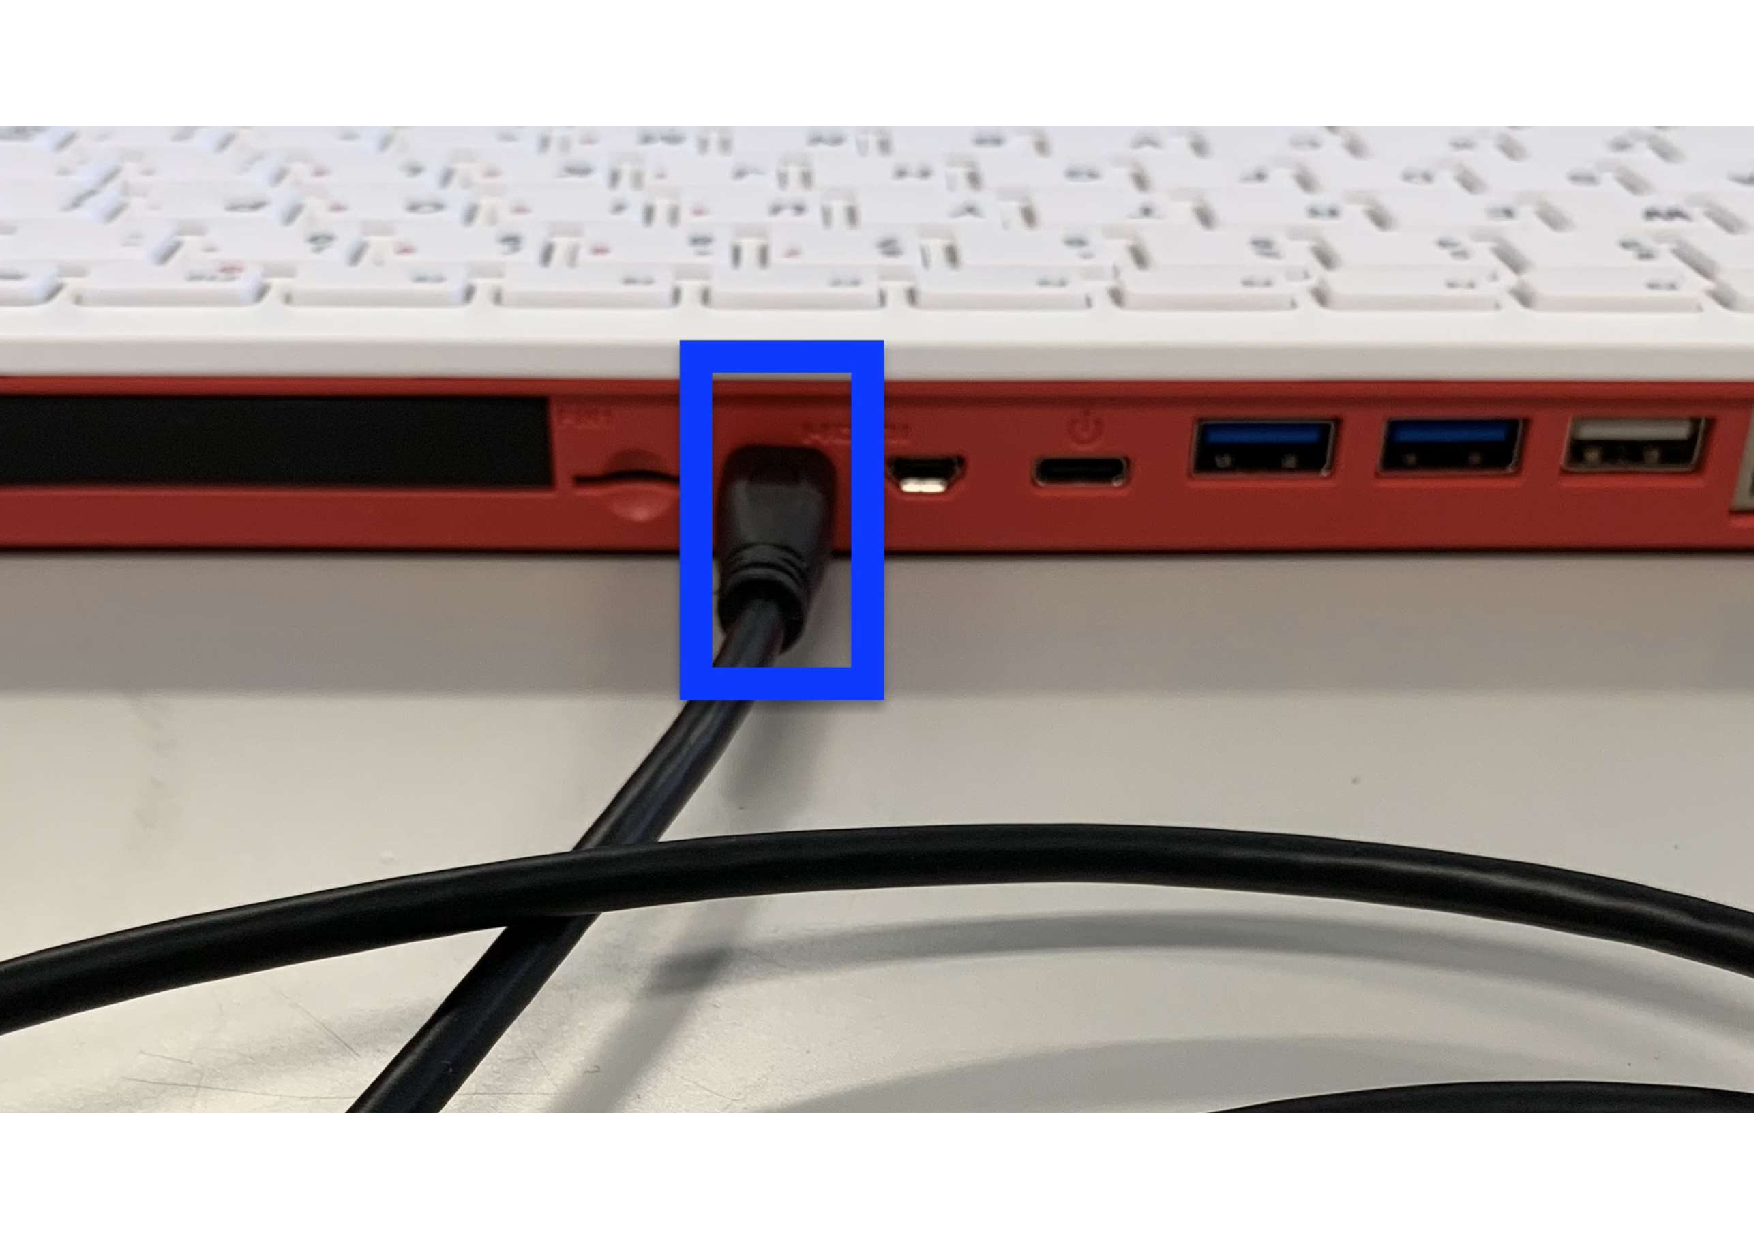
\includegraphics[height=3.471cm]{text01-img/figure222023.pdf}
            \caption{ラズベリーパイHDMI接続}
            \label{fig:2}
          \end{minipage}
  
          \begin{minipage}{0.45\textwidth}
            \centering
            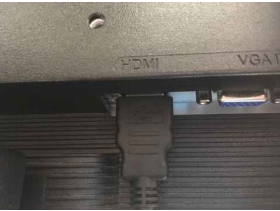
\includegraphics[height=3.471cm]{text01-img/textbook-img016.png}
            \caption{ディスプレイHDMI接続}
            \label{fig:3}
          \end{minipage}
        \end{tabular}
      \end{figure}
    \end{itemize}



  \item マウスをつなぐ

    \begin{itemize}
      \item マウスの先(USBコネクタ)をラズベリーパイへ差し\ruby{込}{こ}みます。
            さす方向に注意してください。
      \begin{figure}[H]
        \centering
        \begin{minipage}{0.5\textwidth}
          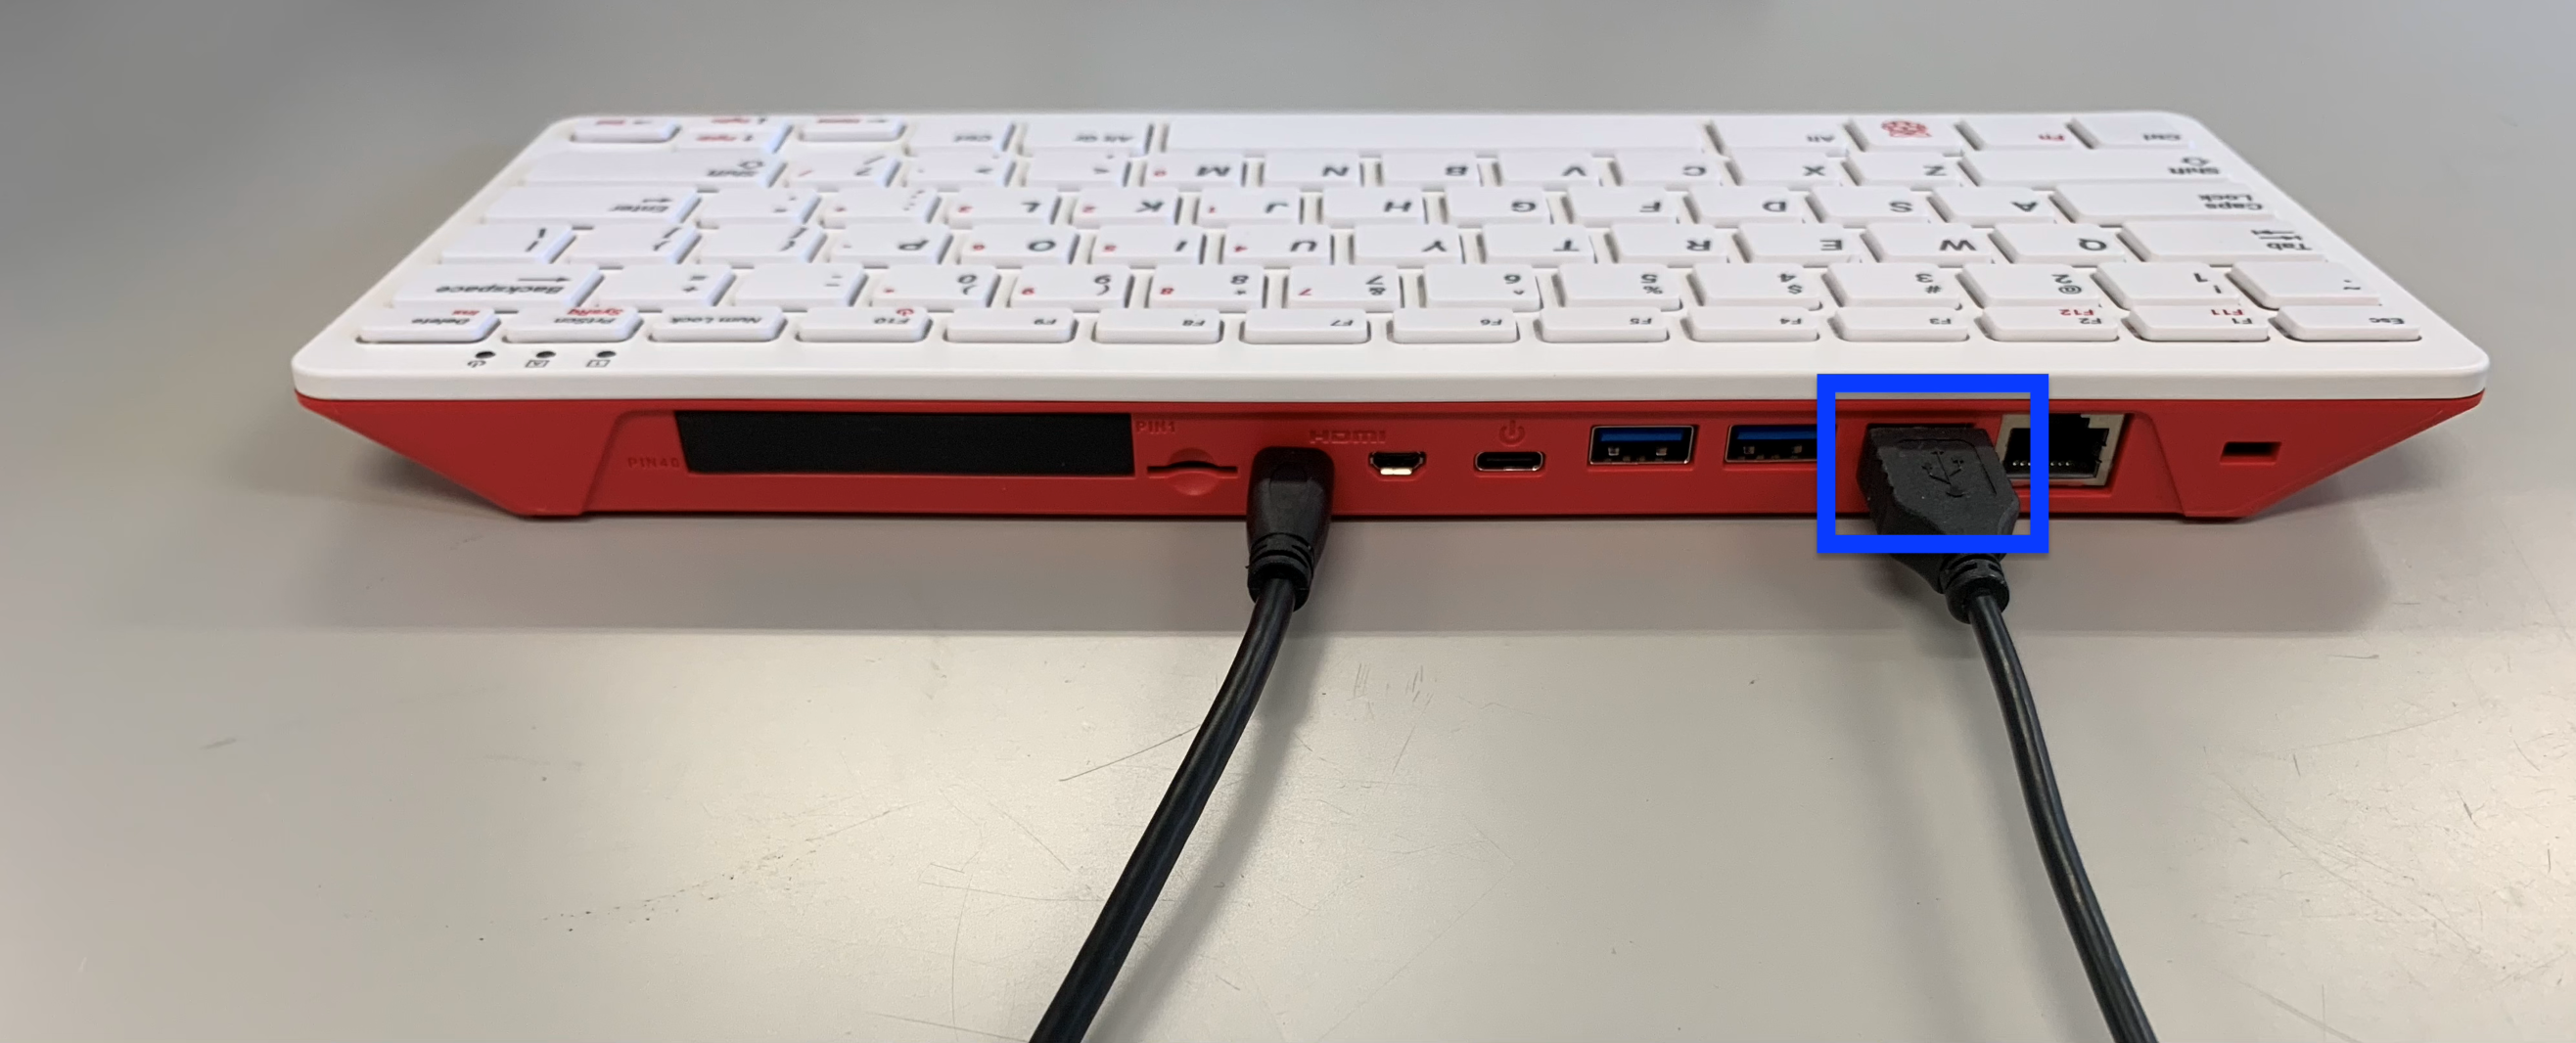
\includegraphics[width=\linewidth]{text01-img/figure1.10-4.png}
          \caption{マウスの\ruby{接続}{せつぞく}}
        \end{minipage}
      \end{figure}
    \end{itemize}
  
  \item microSD(マイクロエスディー)カードをいれる
  
    \begin{itemize}
      \item microSDカードをラズベリーパイ本体にさします。さす方向に注意してください。小さいのでなくさないように気をつけましょう。
      \begin{figure}[H]
        \centering
        \begin{minipage}{0.45\textwidth}
          \includegraphics[width=0.8\linewidth]{text01-img/figure1.10-5.png}
          \caption{microSDカードのさしこみ}
        \end{minipage}
      \end{figure}
    \end{itemize}

  \item モニタの\ruby{電源}{でんげん}をいれる
  
    \begin{itemize}
      \item 次にモニタのコンセントをさします。
      モニタの右はじのボタンをおします。
      でんげんが入ると青色にてんとうします。
      お家でやるときは\ruby{電源}{でんげん}をいれた後に、入力きりかえが必要となる場合がありますので、
      説明書等を\ruby{別途}{べっと}参照してください。
      
      \begin{figure}[h]
        \centering
        \begin{minipage}{0.45\textwidth}
          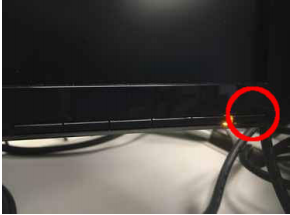
\includegraphics[width=0.8\linewidth]{text01-img/textbook-img019.png}
          \caption{モニタでんげんボタンの位置}
        \end{minipage}
      \end{figure}
    \end{itemize}

  \item ラズベリーパイの\ruby{電源}{でんげん}をいれる
  
    \begin{itemize}
      \item 最後にラズベリーパイのでんげんをいれます。
      図~\ref{fig:7}のようにラズベリーパイにでんげんケーブルをさしてコンセントへ\ruby{接続}{せつぞく}します。
      緑色のランプがついてディスプレイにラズベリーが\ruby{表示}{ひょうじ}がされます 図~\ref{fig:8}。
      
      \begin{figure}[H]
        \begin{tabular}{cc}
          \begin{minipage}{0.45\textwidth}
            \centering
            \includegraphics[width=0.8\linewidth]{text01-img/textbook-img020-2023.png}
            \caption{ラズベリーパイでんげん\ruby{接続}{せつぞく}}\label{fig:7}
          \end{minipage}
  
          \begin{minipage}{0.45\textwidth}
            \centering
            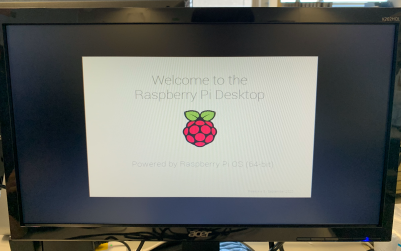
\includegraphics[width=0.8\linewidth]{text01-img/textbook-img0212023.png}
            \caption{ラズベリーパイ起動中}\label{fig:8}
          \end{minipage}
        \end{tabular}
      \end{figure}

    \end{itemize}

\end{enumerate}
\clearpage


% 
% subsection
% 
\subsection*{例題 1-1 セットアップをしよう}
  \begin{itemize}
    \item 定住国を\ruby{設定}{せってい}して言語とタイムゾーンを決定します
    \item raspberry pi 400 が起動すると,このような図~\ref{fig:9}セットアップの開始画面になります。この画面では
    そのままNextのボタンを\ruby{押}{お}して次に進みます。
  \end{itemize}
  \begin{figure}[h]
    \centering
    \begin{minipage}{0.5\textwidth}
      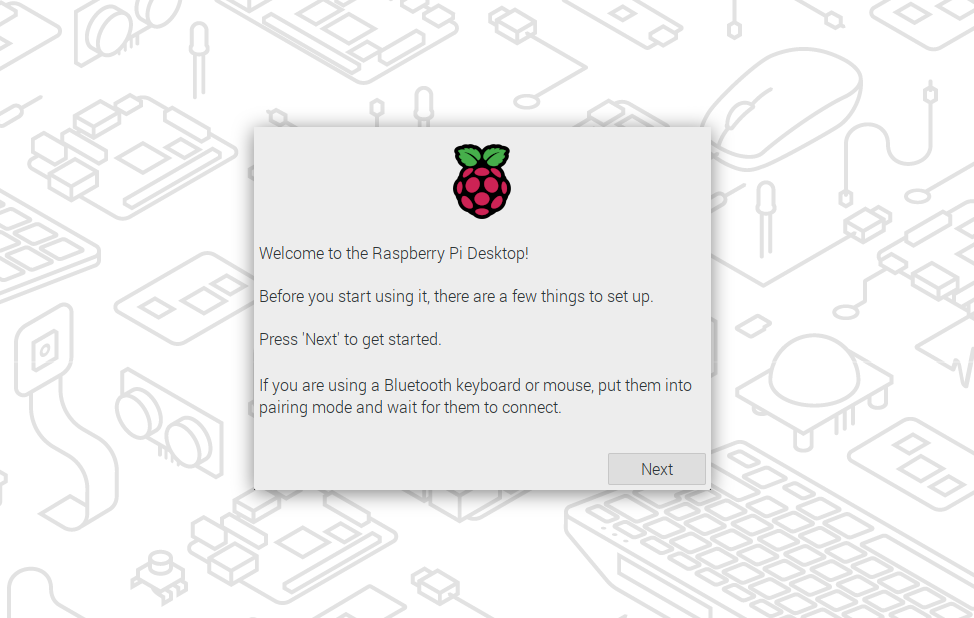
\includegraphics[width=0.9\linewidth]{text01-img/sw_image01.png}
      \caption{起動後画面}\label{fig:9}
    \end{minipage}
  \end{figure}

  \begin{itemize}
    \item 次の画面では図~\ref{fig:10}のように自分の住んでいる\ruby{地域}{ちいき}(タイムゾーン)を\ruby{設定}{せってい}することで
    言語や時間を決定することができます。
    今回は\ruby{皆}{みな}さん日本に住んでいると思うのでcountryの行をクリックすると図~\ref{fig:11}のように\ruby{様々}{さまざま}な
    国の名前が\ruby{表示}{ひょうじ}されるのでその中からJapanを\ruby{選択}{せんたく}してください。
    そうすると他のLanguage, Timezoneの\ruby{項目}{こうもく}がjapanese,Tokyoになります。
    これらはそれぞれ言語とタイムゾーンを表しています。
    それぞれJapan,japanese, Tokyoになっていることとピンクの\ruby{枠}{わく}の場所にチェックが入っていることを
    \ruby{確認}{かくにん}できたらNextボタンを\ruby{押}{お}します。
  
    \begin{figure}[h]
      \centering
      \begin{tabular}{cc}
        \centering
        \begin{minipage}{0.45\textwidth}
          \centering
          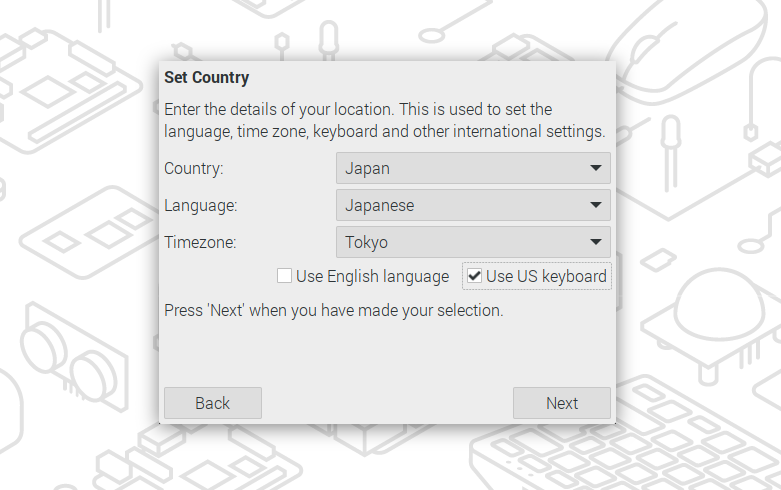
\includegraphics[width=\linewidth]{text01-img/sw_image02.png}
          \caption{タイムゾーン画面}\label{fig:10}
        \end{minipage}

        \begin{minipage}{0.45\textwidth}
          \centering
          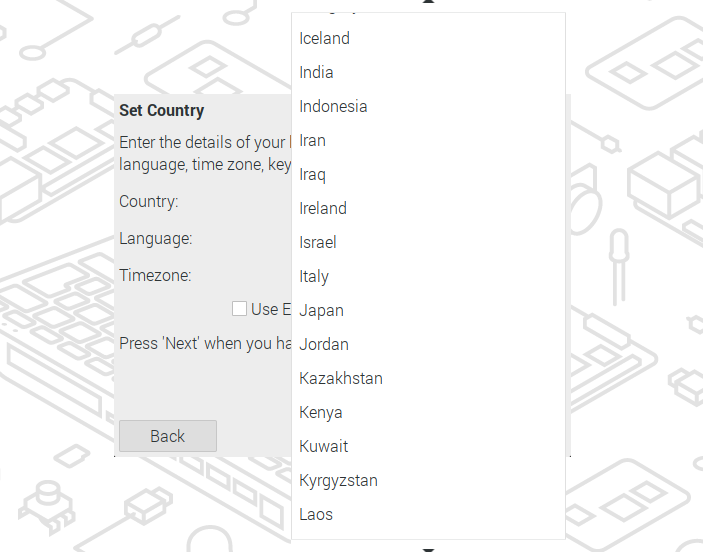
\includegraphics[width=\linewidth]{text01-img/sw_image03-2.png}
          \caption{\ruby{選択}{せんたく}画面}\label{fig:11}
        \end{minipage}
      \end{tabular}
    \end{figure}

    \item 注意点として\ruby{未来塾}{みらいじゅく}で使用するキーボードの配列について\ruby{日常的}{にちじょうてき}に
    日本で使用されているキーボードの配列とは\ruby{異}{こと}なるコンピュータの\ruby{専門家}{せんもんか}に多く使われている
    米国のUS配列というキーボードを用いています。
    キーボードの\ruby{並}{なら}びは国や\ruby{規格}{きかく}、機械などによってそれぞれ\ruby{異}{こと}なった形を持つものがあるので
    注意してください。 
  \end{itemize}  

\clearpage 

% 
% subsection
% 
\subsection*{例題 1-2 パスワードとユーザー名(ID)を決めよう}
\begin{itemize}
  \item 次にユーザーを作成します。図~\ref{fig:12}のように上から順にユーザー名、パスワード、\ruby{再度}{さいど}入力用パスワードの入力の順になっています。
  
  \begin{figure}[h]
    \centering
    \begin{minipage}{5.228cm}
      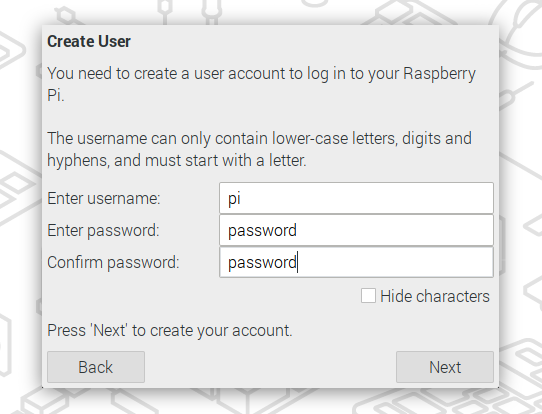
\includegraphics[width=6.000cm]{text01-img/sw_image03.png}
      \caption{ユーザー作成}\label{fig:12}
    \end{minipage}
  \end{figure}

  \item  先ほど記入したものを\ruby{実際}{じっさい}に入力してみます。その\ruby{際}{さい}にこのような画面図~\ref{fig:13}が出てきたらユーザー名(ID)かパスワードのどれかに不正な文字などが\ruby{含}{ふく}まれている\ruby{可能性}{かのうせい}があるのでもう一度\ruby{確認}{かくにん}しましょう。
  
  \begin{figure}[h]
    \centering
    \begin{minipage}{5.228cm}
      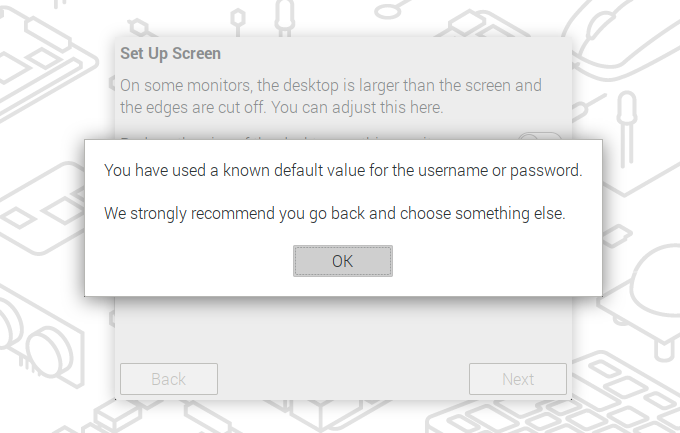
\includegraphics[width=6.000cm]{text01-img/sw_image04.png}
      \caption{エラー画面}\label{fig:13}
    \end{minipage}
  \end{figure}

  % \item 次にスクリーンサイズをTAの人と画面が\ruby{歪}{ゆが}んだりしていないか、\ruby{縦横}{たてよこ}に\ruby{伸}{の}びていないかを\ruby{一緒}{いっしょ}に\ruby{確認}{かくにん}してください。問題の無い場合はNextを\ruby{押}{お}して次に進みます。図~\ref{fig:14}
  
  % \begin{figure}[h]
  %   \centering
  %   \begin{minipage}{5.228cm}
  %     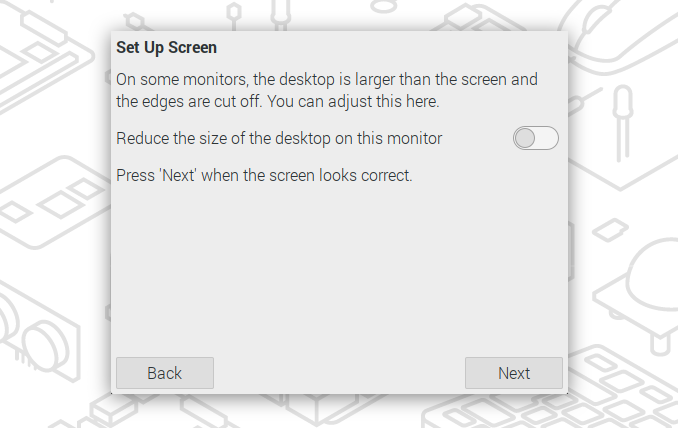
\includegraphics[width=6.000cm]{text01-img/sw_image05.png}
  %     \caption{スクリーンサイズ\ruby{確認}{かくにん}}\label{fig:14}
  %   \end{minipage}
  % \end{figure}

\end{itemize}
\clearpage



% 
% subsection
% 
\subsection*{例題 1-3 Wi-Fiを\ruby{接続}{せつぞく}しよう}
\begin{itemize}
  \item 次にWi-Fiの\ruby{設定}{せってい}を行います。この\ruby{赤枠}{あかわく}の中に\ruby{接続可能}{せつぞくかのう}なWi-Fiの名前が\ruby{表示}{ひょうじ}されます。図~\ref{fig:15}
  \item \textbf{問題 1-5} またこのセクションではWi-FIのアドレスとパスワードが必要となるのでTA(ティーチングアシスタント(Teaching Assistant))の人からアドレスとパスワードを教えてもらい、下の\ruby{欄}{らん}に記入しておきましょう。
  \vskip\baselineskip
  \vskip\baselineskip
  \vskip\baselineskip
  \underline{Wi-Fiアドレス:\hspace{10.7cm}}
  \vskip\baselineskip
  \vskip\baselineskip
  \vskip\baselineskip
  \vskip\baselineskip
  \underline{パスワード:\hspace{11.3cm}}
  \vskip\baselineskip

  % \addBlank{Wi-Fiアドレス}%後で修正
  % \addBlank{パスワード}%後で修正
  
  \item 上部で記入したアドレスを\ruby{選択}{せんたく}してNextのボタンを\ruby{押}{お}します。
  \begin{figure}[H]
    \centering
    \begin{minipage}{5.228cm}
      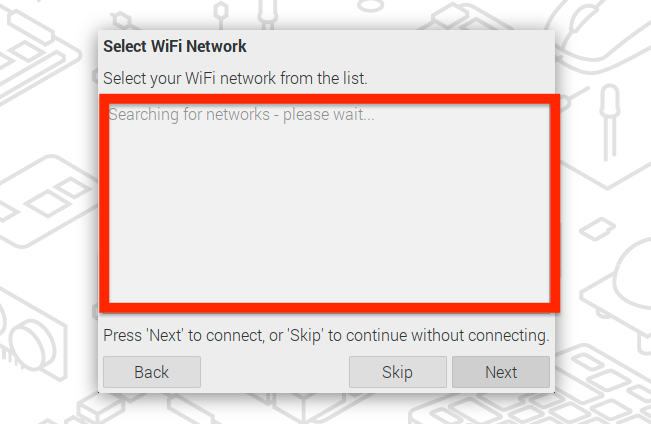
\includegraphics[width=7.000cm]{text01-img/sw_image06kai.png}
      \caption{Wi-Fi\ruby{設定}{せってい}}\label{fig:15}
    \end{minipage}
  \end{figure}

  \item そうするとパスワードを入力するように求められます。 ここでも上部で記入したパスワードを入力してNextを\ruby{押}{お}します。
  \begin{figure}[H]
    \centering
    \begin{minipage}{5.228cm}
      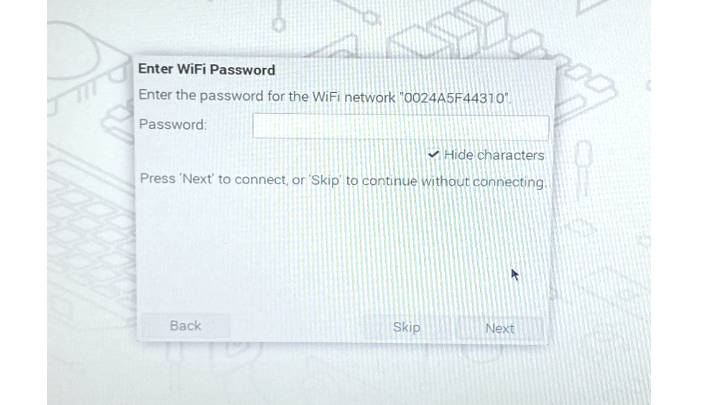
\includegraphics[width=9.000cm]{text01-img/pswd_image_0404.png}
      \caption{パスワード入力}
    \end{minipage}
  \end{figure}
\end{itemize}
\clearpage


% \subsection{ブラウザを選択しよう}

% 
% subsection
% 
\subsection*{例題 1-4 アップデートをスキップしてraspberry piを始めよう}
\begin{itemize}
  \item まず、デフォルトのブラウザを選択します。ここでは図~\ref{fig:16x}の赤い枠のFirefoxを\ruby{選択}{せんたく}して、Nextのボタンを\ruby{押}{お}します。
  \begin{figure}[h]
    \centering
    \begin{minipage}{5.228cm}
      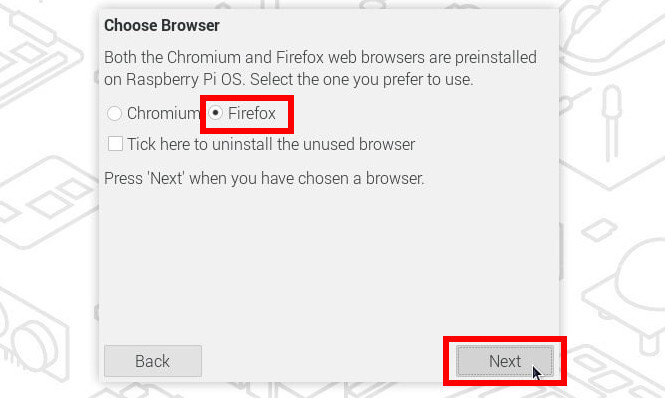
\includegraphics[width=7.000cm]{text01-img/2024_image01.jpg}
      \caption{ブラウザの選択}\label{fig:16x}
    \end{minipage}
  \end{figure}
\end{itemize}

\begin{itemize}
  \item 次の画面に進むとソフトウェアアップデートを求められますが、
  \textbf{今回はアップデートをしないでください。図~\ref{fig:17}の}\textbf{\color{red}赤い枠のSkipボタン}を
  \ruby{押}{お}して次の画面に\ruby{移動}{いどう}します。
  \begin{figure}[h]
    \centering
    \begin{minipage}{5.228cm}
      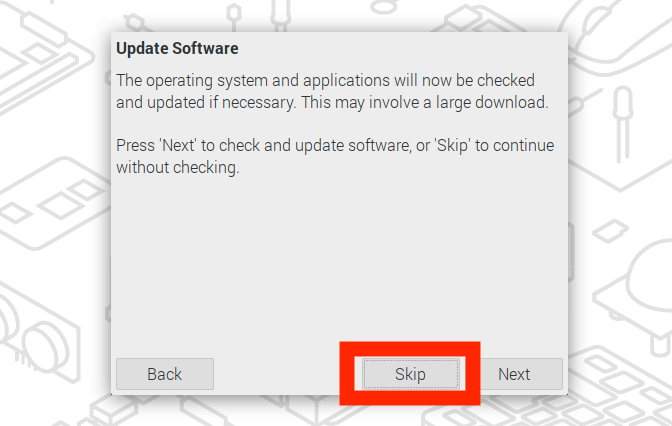
\includegraphics[width=7.000cm]{text01-img/sw_image07.png}
      \caption{ソフトウェアアップデート}\label{fig:17}
    \end{minipage}
  \end{figure}
  \\ここでアップデートをしてしまうと、\ruby{授業}{じゅぎょう}で使う教材の一部が正しく動かなくなってしまいます。
  もし、\ruby{間違}{まちが}えてアップデートをしてしまった場合には、
  SDカードの\ruby{交換}{こうかん}をする必要があるので、すぐにグループの先生に\ruby{相談}{そうだん}してください。
\end{itemize}
\clearpage

\begin{itemize}
  \item \ruby{再起動}{さいきどう}してraspberry piを始めよう
  \begin{itemize}
    \item 次に大まかな初期\ruby{設定}{せってい}が\ruby{完了}{かんりょう}したので\ruby{再起動}{さいきどう}を行います。
    画面右下にあるRestartのボタンを\ruby{押}{お}してください。
    そうすると\ruby{再起動}{さいきどう}が開始されます。
    \begin{figure}[h]
      \centering
      \begin{minipage}{5.228cm}
        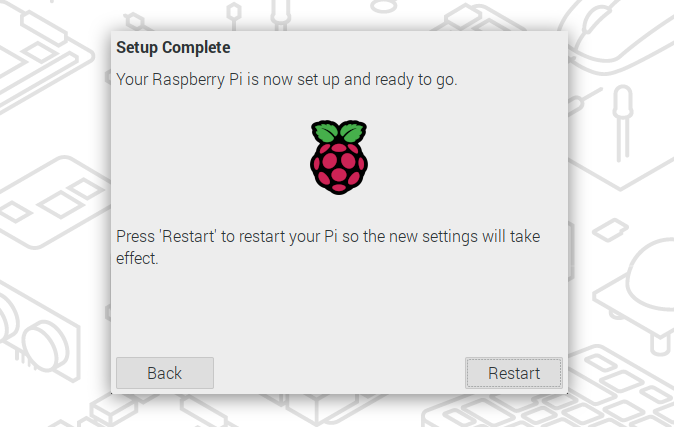
\includegraphics[width=7.000cm]{text01-img/sw_image08.png}
        \caption{\ruby{再起動}{さいきどう} }
      \end{minipage}
    \end{figure}
  \end{itemize}
\end{itemize}



